\documentclass[sigconf,review,screen]{acmart}




\usepackage{wasysym}
\usepackage{graphicx}
\usepackage{balance}  % for  \balance command ON LAST PAGE  (only there!)
\usepackage{amsmath}
%\usepackage{amssymb}
\usepackage{microtype}
\usepackage{booktabs}
\usepackage{etex}

\usepackage{wrapfig}
\usepackage{enumitem}
\usepackage{listings}
\usepackage[english]{babel}
\usepackage{multirow}
\usepackage{times}
\usepackage{tabularx}
\usepackage{verbatim}
\usepackage{caption}
\usepackage{subcaption}
\usepackage[export]{adjustbox}
\usepackage[utf8]{inputenc}
\usepackage[ruled,vlined,linesnumbered]{algorithm2e}%
\usepackage{etoolbox}
\usepackage{tcolorbox}
\usepackage{xcolor}
\usepackage[colorinlistoftodos]{todonotes}
\usepackage{bbm}
\usepackage[flushleft]{threeparttable}
\DeclareMathOperator{\poly}{\textup{poly}}

\usepackage{etoolbox}
\usepackage{marginnote}
\usepackage{soulutf8}
\soulregister{\cite}{7} % Register \cite command with soul
\soulregister{\emph}{7} % Register \cite command with
\soulregister{\autoref}{7} % Register \cite command


\makeatletter
\newcommand{\removelatexerror}{\let\@latex@error\@gobble}
\patchcmd{\SOUL@ulunderline}{\dimen@}{\SOUL@dimen}{}{}
\patchcmd{\SOUL@ulunderline}{\dimen@}{\SOUL@dimen}{}{}
\patchcmd{\SOUL@ulunderline}{\dimen@}{\SOUL@dimen}{}{}
\patchcmd{\SOUL@ulunderline}{\dimen@}{\SOUL@dimen}{}{}
\newdimen\SOUL@dimen
\makeatother
%
\sethlcolor{yellow!20}

% \DeclareRobustCommand{\update}[3][0em]{\marginnote{#2}[#1]\hl{#3}}
\DeclareRobustCommand{\update}[3][0em]
\makeatother


\newcommand{\code}[1]{{\textsf{{\small #1}}}}
% \newcommand{\todo}[1]{\textcolor{red}{\textit{#1}}}
\newcommand{\todomargin}[1]{\marginpar{\textcolor{red}{\textit{#1}}}}

\definecolor{forestgreen}{HTML}{228C22}

\renewcommand{\labelitemi}{$\circ$}
\renewcommand{\labelitemii}{$-$}

\def\Snospace~{\S{}}
\renewcommand*\sectionautorefname{\Snospace}
\renewcommand*\subsectionautorefname{\Snospace}
\renewcommand*\algorithmautorefname{Alg.}
\newcommand*\exampleautorefname{Example}
\newcommand*\lemmaautorefname{Lemma}
%\newcommand*\theoremautorefname{Theorem}
\newcommand*\propertyautorefname{Property}
\newcommand*\problemautorefname{Problem}
\newcommand*\definitionautorefname{Def.}
\renewcommand*{\algorithmcflinename}{line}
\renewcommand\equationautorefname{Eq.}
\renewcommand*\figureautorefname{Fig.}


\SetAlgoSkip{}

\newcommand{\exampleboxh}[2]{
\begin{tcolorbox}[colback=white,
	float,
	floatplacement=h,
	enlarge top by=-.6em,
	enlarge bottom by=-.6em,
	colframe=gray!75!black,
	title=\scshape\fontseries{sb}\selectfont#1,
	boxsep=3pt,
	left=1pt,
	right=1pt,
	top=0pt,
	bottom=0pt,
	toptitle=0pt,
	bottomtitle=0pt,
	lefttitle=1pt,
	righttitle=1pt,
	]{\small%
#2%
}
\end{tcolorbox}%
}

\newcommand{\examplebox}[2]{
\begin{tcolorbox}[colback=white,
	float,
	floatplacement=t,
	enlarge bottom by=-.6em,
	colframe=gray!75!black,
	title=\scshape\fontseries{sb}\selectfont#1,
	boxsep=3pt,
	left=1pt,
	right=1pt,
	top=1pt,
	bottom=1pt,
	toptitle=0pt,
	bottomtitle=0pt,
	lefttitle=1pt,
	righttitle=1pt,
	]{\small%
		#2%
	}
\end{tcolorbox}%
}

\newtheorem{corollary}{Corollary}
\newtheorem{problem}{Problem}
\newtheorem{lemma}{Lemma}
\newtheorem{definition}{Definition}
\newtheorem{example}{Example}
\newtheorem{property}{Property}
\newtheorem{theorem}{Theorem}

\lstset{ %
	belowskip=-2em,
	backgroundcolor=\color{white},   % choose the background color; you must
	basicstyle=\footnotesize\ttfamily,        % the size of the fonts that are
	%used
	%for the code
	breakatwhitespace=false,         % sets if automatic breaks should only
	%happen at whitespace
	breaklines=true,                 % sets automatic line breaking
	captionpos=b,                    % sets the caption-position to bottom
	commentstyle=\color{Brown},    % comment style
	deletekeywords={...},            % if you want to delete keywords from the
	%given language
	escapeinside={\%*}{*)},          % if you want to add LaTeX within your code
	extendedchars=true,              % lets you use non-ASCII characters; for
	%8-bits encodings only, does not work with UTF-8
	frame=,                    % adds a frame around the code
	keepspaces=true,                 % keeps spaces in text, useful for keeping
	%indentation of code (possibly needs columns=flexible)
	keywordstyle=\color{ACMDarkBlue},       % keyword style
	language=,                 % the language of the code
	morekeywords={*,RETURN,SEQ,WITHIN,PATTERN,NOT,
		WHERE,AND,NSEQ,ms,h, min, range},
	%
	%if you want to add more keywords to the set
	numbers=none,                    % where to put the line-numbers; possible
	%values are (none, left, right)
	numbersep=5pt,                   % how far the line-numbers are from the
	%code
	numberstyle=\tiny\color{gray}, % the style that is used for the line-numbers
	rulecolor=\color{black},         % if not set, the frame-color may be
	%changed
	%on line-breaks within not-black text (e.g. comments (green here))
	showspaces=false,                % show spaces everywhere adding particular
	%underscores; it overrides 'showstringspaces'
	showstringspaces=false,          % underline spaces within strings only
	showtabs=false,                  % show tabs within strings adding
	%particular
	%underscores
	stepnumber=1,                    % the step between two line-numbers. If
	%it's
	%1, each line will be numbered
	stringstyle=\color{RedOrange},     % string literal style
	tabsize=2,                       % sets default tabsize to 2 spaces
	title=\lstname,                   % show the filename of files included
	%with
	%\lstinputlisting; also try caption instead of title
}



\hypersetup{
	pdftoolbar=true,        % show Acrobat?s toolbar?
	pdfmenubar=true,        % show Acrobat?s menu?
	pdffitwindow=false,     % window fit to page when opened
	pdfstartview={FitH},    % fits the width of the page to the window
	pdftitle={},    % title
	pdfauthor={},     % author
	pdfsubject={},   % subject of the document
	pdfcreator={},   % creator of the document
	pdfproducer={}, % producer of the document
	pdfkeywords={}, % list of
	%keywords
	pdfnewwindow=true,      % links in new window
	colorlinks=true,       % false: boxed links; true: colored links
	  linkcolor=Brown,          % color of internal links (change box color
%	with
%	linkbordercolor)
	  citecolor=OliveGreen,        % color of links to bibliography
	  filecolor=magenta,      % color of file links
	  urlcolor=NavyBlue           % color of external links
}

\newcommand{\sys}{DISCES\xspace}

\renewcommand{\UrlFont}{\ttfamily\scriptsize} %?
\newcommand{\sstitle}[1]{\smallskip\noindent\textbf{#1.\/}}
\newcommand{\sstitlenoskip}[1]{\noindent\textbf{#1.\/}}

\newcommand{\change}[1]{\textcolor{blue}{#1}}


\DeclareMathOperator{\dom}{dom}
\DeclareMathOperator{\argmin}{argmin}

\newcommand\Mark[1]{\textsuperscript#1}
\newcommand{\True}{\mathit{True}}
\newcommand{\False}{\mathit{False}}
\def\ua{\Mark{*}}
\def\ub{\Mark{\dag}}
\def\uc{\Mark{\#}}
\def\ud{\Mark{+}}

\begin{document}
\title{\sys{}: Systematic Discovery of Event Stream Queries}
\subtitle{Technical Report\vspace{1cm}}


%% The "author" command and its associated commands are used to define the
%%authors and their affiliations.
\author{Rebecca Sattler}
\affiliation{%
 \institution{Humboldt-Universit\"at zu Berlin}
 \city{Berlin}
 \country{Germany}
}
\email{rebecca.sattler@informatik.hu-berlin.de}

\author{Sarah Kleest-Meißner}
\affiliation{%
 \institution{Humboldt-Universit\"at zu Berlin}
 \city{Berlin}
 \country{Germany}
}
\email{kleemeis@informatik.hu-berlin.de}

\author{Steven Lange}
\affiliation{%
 \institution{Humboldt-Universit\"at zu Berlin}
 \city{Berlin}
 \country{Germany}
}
\email{langestx@hu-berlin.de}

\author{Markus L. Schmid}
\affiliation{%
	\institution{Humboldt-Universit\"at zu Berlin}
	\city{Berlin}
	\country{Germany}
}
\email{MLSchmid@MLSchmid.de}

\author{Nicole Schweikardt}
\affiliation{%
 \institution{Humboldt-Universit\"at zu Berlin}
 \city{Berlin}
 \country{Germany}
}
\email{schweikn@informatik.hu-berlin.de}

\author{Matthias Weidlich}
\affiliation{%
 \institution{Humboldt-Universit\"at zu Berlin}
 \city{Berlin}
 \country{Germany}
}
\email{matthias.weidlich@hu-berlin.de}



\begin{abstract}
The continuous evaluation of queries over an event stream provides the
foundation for reactive applications in various domains.
Yet, \update{M1\\R1O1}{knowledge of queries that
detect
distinguished event
patterns that are potential causes of the situation of
interest is often not directly available.
However, given a
database of finite, historic
(sub-)streams that have been gathered whenever a situation of interest was
observed, one may aim at automatic discovery of
the respective queries.} Existing algorithms for event query discovery
incorporate ad-hoc design choices, though,  and it is unclear how their
suitability for a database shall be assessed.

In this paper, we address this gap with \sys{}, an algorithmic framework for
event query discovery. \sys{} outlines a design space for discovery algorithms,
thereby making the design choices explicit. We instantiate the
framework to derive four specific algorithms, which all yield correct and
complete results, but differ in their runtime sensitivity. We therefore also
provide guidance on how to select one of the algorithms for a given database
based on a few of its essential properties. Our experiments using simulated and
real-world data illustrate that our algorithms are indeed tailored to databases
showing certain properties and solve the query discovery problem several
orders of magnitude faster than existing approaches.
\end{abstract}

\maketitle


\section{Introduction}
\label{sec:introduction}
Systems for complex event processing (CEP) continuously evaluate a set of
queries over streams of event
data~\cite{DBLP:journals/csur/CugolaM12,DBLP:journals/vldb/GiatrakosAADG20}. As
such, they facilitate the recognition of situations of interest that
materialize as event patterns, thereby enabling reactive and proactive
applications in various domains, including, for instance,
supply chain management~\cite{DBLP:journals/cii/KonovalenkoL19}, urban
transportation~\cite{DBLP:conf/edbt/ArtikisWSBLPBMKMGMGK14}, and
computational finance~\cite{DBLP:journals/computer/ChandramouliAGSR10}.
CEP systems provide a rich model for the
specification of
event queries~\cite{DBLP:conf/debs/ArtikisMUVW17}. Queries typically define
conditions over the attribute values of events to establish their relevance
for a pattern and to correlate them; and they impose constraints on the
ordering of events and their occurrence within a certain window over the
stream.
While event queries enable a comprehensive characterization of a situation of
interest, their specification is challenging in practice. Domain experts may
have a basic understanding of factors that contribute to a
situation that shall be detected by a query, but typically lack full knowledge
about the specific event patterns, in particular in predictive
applications~\cite{DBLP:conf/debs/EngelEF12,DBLP:conf/debs/SejdovicHRS16}.
Here, the occurrence of a
situation (e.g., a delay in a supply chain or a
fraudulent
transaction) is anticipated in order to prevent or mitigate it.
\begin{wrapfigure}{r}{.5\columnwidth}
	\centering
	\vspace{-1em}
	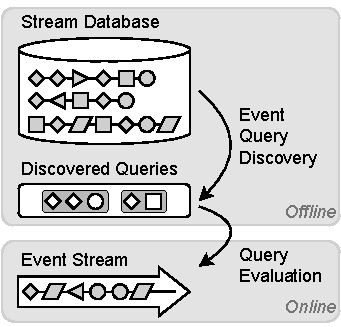
\includegraphics[width=0.5\columnwidth]{img/overview.drawio.pdf}
	\vspace{-2.0em}
	\caption{The general setting.}
	\label{fig:overview}
	\vspace{-1em}
\end{wrapfigure}
To support the specification of event queries, approaches for automated query
discovery have been proposed~\cite{icep,ilminer}. They assume that a database
of finite, historic (sub-)streams, each including at least one
materialization of
the situation, is available, \change{see \autoref{fig:overview}.
Algorithmically discovering queries that match given streams
can generalize historic observations. These resulting queries can
then be reviewed and refined by domain experts before being evaluated
over an event stream to detect future occurrences of the situation of interest.}
Unlike machine learning approaches for pattern detection, the discovery of
event queries provides a traceable and
explainable characterization of a situation of interest.
Solving the problem of event query discovery is computationally hard, though.
The search space of candidate queries grows exponentially in
the query length and the size of the domain of the payload data. Existing
discovery approaches~\cite{icep,ilminer} explore this
space in \emph{one} specific way, which may be suitable for one
database, but leads to intractability for another one. Yet, the assumptions on
the database that motivate the taken design choices are implicit, so that it is
unclear for which database an algorithm can be expected to work.
In this paper, we argue for the systematic design of algorithms for
event query discovery. We aim to answer the following question:
\begin{enumerate}[label=(\roman*),left=0pt,nosep]
\item \emph{What are the design choices in query discovery?}
\item \emph{How to choose a design for a given database?}
\item \emph{How to provide feedback on the algorithmic performance?}
\end{enumerate}
We address these questions through three contributions that we summarize,
along
with the paper structure following a problem formalization
(\autoref{sec:problem}), as follows:
\begin{enumerate}[left=0pt,nosep]
\item We present \sys{} (\autoref{sec:framework})
as a framework
for the design of algorithms for event query
discovery. It captures a set of fundamental design
choices to define discovery algorithms.
\item We instantiate the framework to derive four
discovery algorithms
(\autoref{sec:algos}). They all provide correct
and complete results, yet they differ in their exploration of the space of
candidate queries.
\item We provide means to guide event query discovery
(\autoref{sec:instantiation}). First, we show how to choose among our
algorithms based on a few essential properties of a given stream database.
Second, we provide hints on how to resolve intractability or ineffectiveness of
discovery based on abstractions of the events' payload data.
\end{enumerate}
We evaluated our techniques in experiments using simulated and
real-world data (\autoref{sec:evaluation}). Our results illustrate that the
algorithms designed as part of
the \sys{} framework are indeed tailored to databases that show certain
properties. They solve the query discovery problem
several orders of magnitude faster than existing approaches,
with runtimes that are comparable to
strategies that approximate the result.
We close with a review of related work (\autoref{sec:related_work}) and
conclusions (\autoref{sec:conclusions}).
\section{Problem Setting}
\label{sec:problem}

Below, we
introduce a model for queries over event streams
(\autoref{sec:streams}),
before turning to the problem of query discovery
(\autoref{sec:discovery}).



\subsection{Event Streams and Queries}
\label{sec:streams}


\sstitlenoskip{Event streams}
We adopt a model of multivariate event streams, similar to the one
of relational data stream
processing~\cite{DBLP:journals/vldb/ArasuBW06}. It is
based on the
notion of an \update{M8\\R2O2}{\textbf{event schema}}, which is a tuple of
attributes
$\mathcal{A}= (A_1, \ldots, A_n)$. Each attribute $A_i$, $1\leq i\leq
n$, is of a primitive data type, for which the finite domain is denoted by
$\dom(A_i)$.

Without loss of generality, we assume that all events have a single schema
and that all domains
are distinct, i.e., $\cap_{i=1}^n \dom(A_i) =
\emptyset$. If events actually have different
attributes, they may
be modelled with an event
schema that is the union of all possible attributes, assigning a dedicated
symbol that is ignored in the discovery process to attributes that are not
set.
The schema includes an alphabet $\Gamma =
\bigcup_{i=1}^n{\dom(A_i)}$, i.e.,
the set of all attribute values.
An \update{M8\\R2O2}{\textbf{event}} $e=(a_1, \ldots, a_n)$ is a tuple of
attribute
values that instantiates the event schema, i.e., $a_i\in \dom(A_i)$ for $1\leq
i\leq n$, and we write
$e.A_i$ to refer to the value of attribute $A_i$ of event $e$.
The starting point for query discovery is an \update{}{\textbf{event
stream}}, a finite
sequence of events $S=\langle e_1, \ldots, e_l
\rangle$ {that are ordered by their occurrence time,
with $|S|$
denoting its length. It represents a
finite subsequence recorded of a
potentially unbounded sequence of events.}
Here, we write $S[i]$ for the $i$-th
event in the stream. A \update{}{\textbf{stream database}} is a set
of
streams $D=\{S_1,\ldots, S_d\}$, which may overlap in their contained events.
A stream database $D$ induces the supported stream alphabet
$\Gamma_D \subseteq \Gamma$, containing all values that occur in every stream,
i.e.,

$\Gamma_D = \{a \in \Gamma \mid \forall \ S \in D: \exists \
j\in\{1,\dots,|S|\}, i\in\{1,\dots,n\}: S[j].A_i = a\}$.

\sstitle{Event queries}

Queries over event streams describe sequences of events that are
correlated by predicates over their attribute
values~\cite{DBLP:conf/sigmod/ZhangDI14,DBLP:journals/vldb/GiatrakosAADG20}.
While many models include a time window for event occurrences, in our
setting, the temporal
context is induced by the streams of a database.
{Hence, we
do not model a time window explicitly, but note that it may be derived from
the maximal time difference of events observed in one of the streams.}


To capture event queries, we adopt a linearized
representation,
inspired by~\cite{DBLP:conf/btw/Kleest-Meissner23},
that is well suited to describe discovery algorithms.
Let $\mathcal{A} =
(A_1, \ldots, A_n)$ be an event schema, $\mathcal{X}$ a finite set of variables
with $\mathcal{X}\cap
\Gamma=\emptyset$, and $\_ \notin \mathcal{X}\cup
\Gamma$ a placeholder symbol. Then, a \update{M8\\R2O2}{\textbf{query term}}
$t=(u_{1},\ldots,u_{n})$ is an $n$-tuple built of attribute
values, variables, and placeholders, i.e.,
$u_{j}\in \dom(A_j) \cup \mathcal{X} \cup \{ \_ \}$, $1\leq j\leq n$, such that
not all its components are placeholders, i.e., it holds that $u_{j}\in
\dom(A_j) \cup \mathcal{X}$ for at least one $1\leq j\leq n$.
The empty query term $\varepsilon$ is the $n$-tuple comprising only
placeholders, i.e., 
$\varepsilon=(\_,\dots,\_)$.
An event
query is a finite sequence of query terms, $q=\langle t_1,\ldots,t_k \rangle$,
with $q[i]$ denoting the $i$-th term. In a query, variables need to occur in at
least two query terms for the same attribute, i.e., for any term
$q[i]=(u_{1},\ldots,u_{n})$ with $u_j\in \mathcal{X}$,
$1\leq i\leq k$ and $1\leq j\leq n$, there exists another query term
$q[p]=(u'_{1},\ldots,u'_{n})$ with $u_j = u'_j$,
$1\leq p\leq k$ and $p\neq i$. The \update{M8\\R2O2}{\textbf{empty query}}
$\langle\varepsilon\rangle$ contains only the empty query term.
The universe of all possible queries is $\mathcal{Q}$.




Intuitively, each query term characterizes an event that should be matched by
the query. For each attribute, the term enforces a distinct value or
permits any value of the respective domain. In the latter case, a placeholder
models the absence of a constraint, whereas a variable that is used multiple
times enforces equal attribute values.
This way, equivalence
predicates over attributes of events are modelled.


Queries built of terms that contain only attribute values (and
placeholders) are called \update{M8\\R2O2}{\textbf{type queries}}; those
built of terms of only
variables (and placeholders) are called \update{}{\textbf{pattern queries}};
while those
that combine attribute values and variables are called
\update{}{\textbf{mixed queries}}.



To define the query semantics,

let $q=\langle t_1,\ldots,t_k \rangle$ be an event query and
let $S=\langle e_1, \ldots , e_l\rangle$ be an event stream.
A \update{}{\textbf{match}} of $q$ in $S$ is an injective mapping
$m: \{1,\ldots,k\}\rightarrow \{1, \ldots, l\}$,
such that:
\begin{itemize}[nosep,left=1em]
	\item for each query term $q[i]=(u_{1},\ldots,u_{n})$, $1\leq i\leq k$, the
	mapped event $S[m(i)]=(a_1,\ldots, a_n)$ has the required
	attribute
	values, i.e., $u_j = a_j$ or $u_j\in \mathcal{X}\cup \{\_ \}$
	for $1\leq 	j\leq n$;
	\item variables are bound to the same attribute values, i.e., for query
	terms $q[i]=(u_1,\ldots, u_n)$ and $q[p]=(u'_1,\ldots, u'_n)$, $1\leq
	i,p\leq k$, it holds that $u_j\in \mathcal{X}$, $1\leq j\leq n$, with
	$u_j=u'_j$ implies that $S[m(i)].A_j = S[m(p)].A_j$; and
 	\item the order of the events in the stream is preserved,
 	i.e., for $1\leq
	i<p\leq k$, it holds $m(i)<m(p)$.

\end{itemize}
If there exists a match for query $q$ in stream $S$, we say that
$S$ supports $q$ ($q$ matches $S$); and write $S \models q$.

\autoref{tab:notations} lists our notations.


\begin{example}
\label{ex1}
\update{{\normalfont M4\\R1O1\\R2O1}}{
Taking up the example from \autoref{fig:overview}, the stream database is
represented in our models as follows:}
\begin{center}
	{\footnotesize
		\begin{tabular}{l@{\hspace{.5em}}l@{\hspace{.5em}}l@{\hspace{.5em}}l@{\hspace{.5em}}l}
			\toprule
			Stream & Event &  Job &  Status
&  Prio\\
			\midrule
			$S_1$ & $e_{11}$   & 1 & schedule &
low  \\
			 & $e_{12}$   & 1 & kill & low  \\
			 & $e_{13}$   & 1 & schedule & high  \\
			 & $e_{14}$   & 1 & update & high  \\
			\midrule
			$S_2$ & $e_{21}$   & 2 & schedule &
low  \\
			 & $e_{22}$   & 3 & schedule & high  \\
			 & $e_{23}$   & 2 & evict & low  \\

			\bottomrule
	\end{tabular}\quad
		\begin{tabular}{l@{\hspace{.5em}}l@{\hspace{.5em}}l@{\hspace{.5em}}l@{\hspace{.5em}}l}
			\toprule
			Stream & Event &  Job &  Status
&  Prio\\
			\midrule

			$S_3$ & $e_{31}$   & 4 & schedule &
high  \\
			 & $e_{32}$   & 5 & schedule & low  \\
			 & $e_{33}$   & 4 & finish & high  \\
			 & $e_{34}$   & 6 & schedule & low  \\
			 & $e_{35}$   & 5 & evict & low  \\
			\bottomrule
			\vspace{1.8em}
	\end{tabular}
	}
	\end{center}
The query $q = \langle
(x_0,\_,\_),(\_,\_,\text{high}),(x_0,\text{evict},\_) \rangle$
describes three consecutive events (but not necessarily \emph{immediately}
consecutive) in which the first and the last event have the same job id,
the priority of the second event is high and the status of the last event is
evict.
The query does not match $S_1$. It matches $S_2$ and $S_3$, with $e_{21},
e_{22}, e_{23}$ and $e_{32},e_{33},e_{35}$, respectively.
\end{example}



\subsection{Query Discovery}
\label{sec:discovery}

Given a stream database, the problem of event query discovery relates to
the identification of event queries that are supported by all streams, i.e., for
which there exists at least a single match for each stream.

However, there may exist queries that are
supported
by all streams, but which are comparable in the sense that one of them
is stricter than another one. Formally, a query $q$ is defined as stricter
than a query $q'$, denoted by $q\prec q'$, if

(i) for any possible stream $S$ (not necessarily contained in a given stream
database), $S \models q$ implies $S
\models q'$, and (ii) there exists a stream $S$, such that $S \models q'$,
but $S \not\models q$.

In event query discovery, we are only interested in the strictest queries
that are supported by all streams. The reason being that these queries
denote the most {concise} characterization of the
patterns linked to a situation of interest. For a stream database $D$, we
therefore
consider a notion of descriptiveness~\cite{icdt2022}: A query $q$ is
\update{}{\textbf{descriptive}} \update{M8\\R2O2}{}for $D$,
if it is supported by $D$ and
there does not exist a query $q'$ that is stricter, $q'\prec q$, and that is
also supported by the stream database $D$.
Based thereon, we formulate the problem of event query discovery:

\begin{problem}[Event Query Discovery]
\label{problem}
Given a stream database $D=\{S_1,\ldots, S_d\}$,
the problem of event query discovery is to construct the set of queries $Q$,
such that:
\begin{itemize}[nosep,left=1em]
  \item ${Q}$ is correct: each $q\in Q$ creates at least a single match for
  all streams, i.e., for all $q\in Q$ and $S\in D$ it holds that $S \models
  q$;
  \item ${Q}$ is descriptive: only the strictest queries are considered,
  i.e., for all $q,q'\in Q$ it holds that neither $q\prec q'$ nor $q'\prec q$;
  \item ${Q}$ is complete: if a query $q$ is both correct and descriptive,
  then it holds that $q\in Q$, {i.e., ${Q}$ contains
  all queries
  that are both correct and descriptive.}
  \end{itemize}
\end{problem}

\begin{table}[t]
	\caption{Overview of notations.}
	\label{tab:notations}
	\vspace{-1.1em}
	\footnotesize
	\begin{tabularx}{0.47\textwidth}{l
	@{\hspace{.5em}} p{5.8cm}}
	\toprule
	Notation & Explanation \\
	\midrule
	$\mathcal{A}=(A_1, \ldots, A_n )$ & An event
	schema, a
	tuple of attributes\\
	$\Gamma  = \bigcup_{i=1}^n{\dom(A_i)}$ & The stream alphabet\\
	$e= (a_1, \ldots, a_n)$ & An event, a tuple
	of attribute values\\
	$e.A_i$ & The value $a_i$ of attribute $A_i$ of
	event $e$\\
	$S=\langle e_1, \ldots, e_l \rangle$ & An event
	stream, a finite sequence of events\\
	$S[i]$ & The $i$-th event of the event stream $S$\\
	$D=\{S_1,\ldots, S_d \}$ & A stream database, a
	set of event streams\\
	$\Gamma_D$ & The supported stream alphabet of stream database $D$\\
	\midrule
	$\mathcal{X}$ & A finite set of query variables, $\mathcal{X} \cap
	\Gamma=\emptyset$\\
	$\_$ & A placeholder symbol, $\_ \notin \mathcal{X}\cup
	\Gamma$\\
	$t=(u_{1},\ldots,u_{n})$& A query term, an
	$n$-tuple of attribute values, variables, and placeholders with $u_{j}\in
	\dom(A_j) \cup \mathcal{X} \cup \{\_ \}$, $1\leq j\leq n$, such that not
	all its components are placeholders\\
	$\varepsilon=(\_,\ldots,\_)$& The empty query term, an
$n$-tuple of placeholders\\
	$q=\langle
	t_1, \ldots, t_k \rangle$ & An event query, a finite sequence of
	query terms \\
	$q[i]$ & The $i$-th term of the query $q$\\
	$\langle \varepsilon\rangle$ & The empty query containing only the empty
	query term \\
	\midrule
	$S \models q$ & The stream $S$ supports the
	query $q$, i.e., there exists a match\\
	
	\bottomrule
	\end{tabularx}
	\vspace{-1.5em}
\end{table}


\begin{example}
Consider the following two queries:
\begin{align*}
    q_1 &= \langle (x_0,\text{schedule},\text{low}),(\_,\_,\text{high}),(x_0,\_,\_)
    \rangle \\
     q_2 &= \langle (x_0,\text{schedule},\text{low}),(x_0,\_,\_) \rangle.
\end{align*}
\update{{\normalfont M4\\R1O1\\R2O1}}{Query $q_1$ is the representation of
the query from \autoref{fig:overview}
in our model.} Both queries match the stream database of \autoref{ex1}.
Also, $q_1$ is stricter than $q_2$: Any stream that matches $q_1$ will
also match $q_2$, but not vice versa. Query $q_1$ is even descriptive

for the given database.
\end{example}

\section{The \sys{} Framework}
\label{sec:framework}
This section introduces \sys{} as a framework for the systematic design of
algorithms to address the problem of event query discovery. We first discuss
dimensions along which design choices are captured (\autoref{sec:dimensions}),
before turning to their combination (\autoref{sec:combinations}).
\begin{table*}
    \smaller
	     \caption{Illustration of the dimensions that are incorporated in
	     the design of
		discovery algorithms as part of the \sys{} framework.}
	\label{fig:dimensions_overview}
	\vspace{-1em}
	\begin{tabular}{crclll|llll|llll|lll}
        \toprule
        \multicolumn{6}{c}{Direction}
                                & \multicolumn{4}{c}{Strategy} &
        \multicolumn{4}{c}{Construction: Separated | Unified} & \multicolumn{3}{c}{Attributes: Separated | Comprehensive} \\
        \midrule
        \multicolumn{5}{c}{$\langle(a,5,11)\rangle$}             &                                                                                                                        &  \multicolumn{1}{l}{\tcbox[colback=white, colframe=black, on line, size=fbox]{\underline{$\langle(a,5)\rangle$}} }  &  &  &  & \multicolumn{1}{c}{{$\langle(x,y),(x,y)\rangle$}} & \multicolumn{1}{c}{{$\langle(a,5)\rangle$}} &   \multicolumn{1}{c}{{$\langle(x,5),(x,\_)\rangle$} }    &      &  \multicolumn{1}{c}{$\langle(x),(a),(x)\rangle$}    & \multicolumn{1}{c}{$\langle(5),(7)\rangle$} &  \multicolumn{1}{c}{$\langle(x,5),(x,7)\rangle$}  \\
        \multicolumn{1}{l}{bottom} & \multirow{2}{*}{$\uparrow$} & \multirow{2}{*}{$\vdots$} & \multirow{2}{*}{$\downarrow$} & top & & \multicolumn{1}{c}
     {$\uparrow$}   &  & & &  \multicolumn{1}{c}{$\uparrow$} &
     \multicolumn{1}{c}{$\uparrow$} & \multicolumn{1}{c}{$\uparrow$}  &  &
     \multicolumn{1}{c}{$\color{black}\uparrow$}  &
     \multicolumn{1}{c}{$\uparrow$} &      \multicolumn{1}{c}{$\uparrow$}
     \\
        \multicolumn{1}{l}{up}     &
        &                           &                               & down
        &  &  \multicolumn{3}{c}{\tcbox[colback=white, colframe=black, on
        line, size=fbox]{\underline{$\langle(a,\_)\rangle$};
        $\langle(\_,5)\rangle$}}             &              &
        \multicolumn{1}{c}{{$\langle(x,\_),(x,\_)\rangle$}} &
        \multicolumn{1}{c}{$\langle(a,\_)\rangle$}&
        \multicolumn{1}{c}{$\langle(x,\_),(x,\_)\rangle$}       &   &
        \multicolumn{1}{c}{$\langle(x),(x)\rangle$}    &
        \multicolumn{1}{c}{$\langle(5)\rangle$} &
        \multicolumn{1}{c}{$\langle(x,5),(x,\_)\rangle$}
        \\[1em]
        \multicolumn{5}{c}{$\langle(a,\_,\_)\rangle$} &
                              & \multicolumn{3}{c}{\underline{DFS} |
        \tcbox[colback=white, colframe=black, on line, size=fbox]{BFS}}  & &
        \multicolumn{1}{c}{\textcolor{black}{pattern queries} } &
        \multicolumn{1}{c}{\textcolor{black}{type queries}}     &
        \multicolumn{1}{c}{\textcolor{black}{mixed queries}}          & &
        \multicolumn{1}{c}{\textcolor{black}{attribute 1}}    &
        \multicolumn{1}{c}{\textcolor{black}{attribute 2}} & all attributes
        \\
        \bottomrule
       \end{tabular}
	\vspace{-1em}
\end{table*}
\subsection{Dimensions of Design Choices}
\label{sec:dimensions}
The \sys{} framework includes four dimensions for design choices that guide how
the space of candidate queries is explored. These dimensions, illustrated in
\autoref{fig:dimensions_overview}, refer to the following properties of the search
through that space, which are detailed in the remainder:
\begin{description}[itemsep=.3em,font=\normalfont\itshape,
labelindent=0em,leftmargin=2.5em]
    \item[Direction:] The search proceeds bottom-up or top-down.
    \item[Strategy:] The approach is depth-first or
    breadth-first.
    \item[Construction:] Type and pattern queries are initially
    constructed separately, or mixed queries are immediately
    considered.
    \item[Attributes:] Attributes are initially considered
    separately, or immediately incorporated comprehensively.
\end{description}
\textbf{Direction.}
When traversing the space of candidate queries, two directions may be considered:
Bottom-up approaches start with the most generic query possible and, by adding
attribute values or variables, generate stricter queries.
The traversal stops, once the sequences in the database no longer support the
explored queries.
Top-down approaches start with a most specific query,
i.e., a shortest \change{stream} of the given database.
Then, they explore the search space by deleting attribute values or exchanging
them with variables; stopping whenever queries that are supported by all sequences
of the database have been found. Considering the example in
\autoref{fig:dimensions_overview}, a bottom-up approach evaluates the query
$\langle (a,\_,\_) \rangle$ before the more specific query $\langle (a,5,11)
\rangle$, and vice versa for a top-down approach.
\textbf{Strategy.} To explore candidate queries, one may adopt a
depth-first search (DFS) strategy. Then, the space is traversed by
generalizing or specializing the queries until a query with a different
support behavior is reached, i.e., a non-supported query is generalized
until it is supported (top-down direction) or a supported query is
specialized until it is no longer supported (bottom-up direction). A
different strategy
is to adopt breadth-first search (BFS), i.e., to first explore all
queries containing an equal number of non-placeholders, before continuing with
those with less (top-down
direction) or more (bottom-up
direction) non-placeholders. In \autoref{fig:dimensions_overview},  assuming a
bottom-up
search direction, from query
$\langle (a,\_) \rangle$, DFS would continue with the stricter query
$\langle (a,5) \rangle$, whereas BFS would first consider queries with the
same number of non-placeholders, such as $\langle (\_,5) \rangle$.
\textbf{Construction.}
Another algorithmic choice is whether to construct type queries and pattern
queries separately or with a unified approach. The former means that the
space of candidate type queries and the space of candidate pattern
queries are explored independently, before merging the results to also
obtain the descriptive mixed queries. Note that the isolated discovery of
type queries corresponds to the common problem of maximal frequent sequence
mining~\cite{10.1007/978-3-319-06483-3_8,10.1007/978-3-642-53914-5_15,10.1145/2757217}.
In a unified approach, in turn, all query structures are explored as part of
a single search space. In \autoref{fig:dimensions_overview}, a separated
approach would explore pattern queries, e.g., $\langle (x,\_),(x,\_) \rangle$
and subsequently $\langle (x,y),(x,y) \rangle$, and type queries, e.g.,
$\langle (a,\_)\rangle$ and then $\langle(a,5) \rangle$ before merging them. A
unified approach would directly construct mixed queries and explore, for
instance, $\langle (x,5),(x,\_)\rangle$ after $\langle (x,\_),(x,\_)\rangle$.
\textbf{Attributes.}
Similarly, the attributes of an event schema induce a
design choice for the exploration of the space of candidate
queries. We may first
explore each attribute separately, before merging the
results to obtain the final set of descriptive queries; or rely on a
comprehensive approach that explores all attributes
simultaneously. Again, \autoref{fig:dimensions_overview} illustrates this
design choice: We may consider the first attribute, exploring $\langle (x),(x)
\rangle$ followed by $\langle (x),(a),(x) \rangle$, and the second attribute,
exploring $\langle (5) \rangle$ followed by $\langle (5),(7) \rangle$ and merging them afterward;
or immediately consider both attributes, by exploring $\langle
(x,5),(x,\_) \rangle$ and then $\langle (x,5),(x,7) \rangle$.
\subsection{Combination of Design Choices}
\label{sec:combinations}
Having described fundamental choices in the design of discovery algorithms,
we review their interplay and underlying assumptions.
First, the choice regarding the search direction, top-down
vs. bottom-up, relates to an important assumption on the application scenario. A
top-down search strategy will commence with a shortest stream of the
database as a query, and step-wise generalize it until queries supported by
the whole database are found. Hence, such an approach can be expected
to work efficiently, if descriptive queries are only slightly shorter than
the shortest stream in the database. In the scenarios outlined
in \autoref{sec:motivation}, however, queries commonly
contain solely a few terms and are generally much shorter than the available
streams. Hence, a top-down exploration of candidate queries will
quickly become intractable, due to the sheer size of the
respective search space. In the remainder, we therefore focus on the
instantiation of algorithms that adopt a bottom-up direction for
the search.
Second, we focus on the combination of search strategies (DFS vs. BFS) and
the construction approach (type/pattern-separated vs. unified). As mentioned
above, the separate construction of type queries and pattern queries enables
us to incorporate existing results: The discovery of type queries in
isolation corresponds to the maximal frequent sequence mining (MFSM)
problem~\cite{agrawal1995}. Since state-of-the-art algorithms for the MFSM
problem rely on BFS,
we adopt it as the search strategy in any approach that is based on the
separate construction of type queries and pattern queries.
In contrast, for the unified construction of queries, a BFS search strategy is
harmful. A bottom-up, unified
construction of queries following BFS will explore mixed queries, for
which it is known that they cannot be descriptive. For instance, the mixed
queries
$\langle (a),(a),(x_0),(x_0)\rangle$ and $\langle (x_0),(x_0),(b),(b) \rangle$ will be
considered as candidates if the queries $\langle (a),(a),(b),(b) \rangle$ and
$\langle (x_0),(x_0),(x_1),(x_1) \rangle$ are supported by the
stream database, even
though the mixed queries cannot be descriptive. A separated construction of
queries avoids the issue, as
does the combination of a unified construction with DFS.
Third, the question whether to consider the attributes
separately or comprehensively is largely orthogonal to the above
design choices. Hence, the separate or comprehensive treatment of attributes
may be combined with either of the above design choices.
Based thereon, we derive the four combinations of design choices
listed in \autoref{tab:algos}, which can be deemed suitable to design
efficient algorithms for the problem of event query discovery.
\begin{table}[h!]
\vspace{-.5em}
\caption{Combination of design choices for discovery algorithms.}
\label{tab:algos}
\vspace{-1em}
\footnotesize
\begin{tabular}{l@{\hspace{1em}} l@{\hspace{1em}} l@{\hspace{1em}}
l@{\hspace{1em}} l}
		\toprule
		& Direction & Strategy & Construction & Attributes \\
		\midrule
		B-S-S & bottom-up & \underline{B}FS & \underline{S}eparated &
		\underline{S}eparated\\
		B-S-C & bottom-up & \underline{B}FS & \underline{S}eparated &
		\underline{C}omprehensive \\
		D-U-S & bottom-up & \underline{D}FS & \underline{U}nified &
		\underline{S}eparated \\
		D-U-C & bottom-up & \underline{D}FS & \underline{U}nified &
		\underline{C}omprehensive \\
		\bottomrule
\end{tabular}
\end{table}

\section{\sys{} Algorithms}
\label{sec:algos}
Having introduced the \sys{} framework to capture important choices in the
design of discovery algorithms, we now turn to its instantiation. We
first introduce algorithms to generate query
candidates (\autoref{sec:candidate}), to match query against a stream
database (\autoref{sec:matching}), and to merge queries
(\autoref{sec:merging}). Based thereon, we propose four specific
discovery algorithms (\autoref{sec:realizations}) that realize the above
design choices.
\subsection{Query Candidate Generation}
\label{sec:candidate}
Our discovery algorithms rely on an iterative generation of query candidates,
which are then matched against a stream database. As detailed in
\autoref{sec:framework}, we follow a
bottom-up direction in the exploration of candidate queries and step-wise
generate stricter queries for a given query $q$. \change{Initially, this
query $q$ is the empty
query, which will be elaborated further later.}
The child queries of $q$ are those obtained by inserting
a new variable, by inserting a variable that has been present already, or by
inserting an attribute value; either way, considering an existing query term
or a newly added query term.
Variables are inserted in a certain order, which
is reflected in a total order $<$ over a set of variables $\mathcal{X}$. To
simplify the notation, we write $\mathcal{X}^<$ for the sequence of
variables induced by $<$ over $\mathcal{X}$. Also, our
construction employs at most $s/2$ variables with $s=\min_{S\in D} |S|$
being the minimal stream length in the stream database. Hence, the size of
$\mathcal{X}$ and the length of $\mathcal{X}^<$ are bounded.
Query candidate generation, formalized in
\autoref{alg-bu-df:childquery}, takes as input a query $q$; an event
schema $\mathcal{A}$; a supported alphabet $\Gamma_D$; a parent dictionary
$P$ that is modelled as a
function $P: \mathcal{Q} \to \mathcal{Q}$, mapping child queries to their
parent; a sequence of variables $\mathcal{X}^<$; and a Boolean flag $b$ to
control whether variables shall be inserted. The algorithm returns the set
of child queries for $q$.
\autoref{alg-bu-df:childquery} is divided into three parts, following an
initialization (\autoref{alg1:init_start} - \ref{alg1:init_end}),
each capturing one type of insertion. It is designed such that \emph{all}
child queries are obtained by
insertion
of a single symbol (attribute value or variable) are constructed
\emph{exactly once}. The generation relies on the auxiliary function
$\textsc{Next}$
(\autoref{alg1:next_start} - \ref{alg1:next_end}). Given a query, it
generates query candidates by inserting a given symbol (variable or attribute value) in
any query term following a given position in the query, if the query
contains a placeholder for that attribute. In addition, it
generates candidates by appending a new query term to the query that
is empty except for the given symbol for the given attribute. Based thereon,
the three parts of the main algorithm include:
\textit{Insertion of a new variable} (\autoref{rule:insertnewvar} -
\ref{rule:insertnewvar_end}). For each attribute, we consider all query
terms after the last occurrence of any attribute value ($g$) and after the first
occurrence of the last inserted variable ($f$). Using function
$\textsc{Next}$, a single new variable $\mathcal{X}^<[v+1]$ is introduced
by replacing a placeholder or adding a new query term.
\begin{figure}[t]
\removelatexerror
\begin{algorithm}[H]
	\footnotesize
	\caption{\textsc{ChildQueries}: Query Cand. Generation}
	\label{alg-bu-df:childquery}
	\KwIn{\, \ Query $q$, event schema $\mathcal{A}$, supported alphabet
		$\Gamma_D$, \\ \hspace{3em} \,
		parent dictionary $P$, sequence of query variables $\mathcal{X}^<$,
		\\ \hspace{3em} \,
		Boolean flag $b\in \{\True,\False \}$ whether to insert variables.
	}
	%\tcc*{some comment}		\;
	\KwOut{Updated parent dictionary $P$.}
	\SetKwFunction{FNext}{\textnormal{\textsc{Next}}}%
	\BlankLine
	$\mathit{g \gets}$ position of last inserted attribute value in $q$\;
	\label{alg1:init_start}
	$\mathit{f \gets}$ first position of last inserted variable in $q$\;
	$z \gets \max(g,f)$\;
	$\mathit{n \leftarrow} |\mathcal{A}|$\;
	\label{alg1:init_end}
	\tcc{\scriptsize Shall variables be inserted?}
	\If{$b= \True$}{
		$v \gets$ number of distinct query variables in $q$\;
		\tcc{\scriptsize Insert a new variable
			$\mathcal{X}^<[v+1]$}
		\ForEach{$A\in\mathcal{A}$}{
			\label{rule:insertnewvar}
			\ForEach{$q'\in
				\FNext(q,z,A,\mathcal{X}^<[v+1],n)$}{
				\label{rule:insertnewvar_step2}
				\ForEach{$q''\in
					\FNext(q',z+|q'|-|q|,A,\mathcal{X}^<[v+1],n)$}{
					$P(q'') \leftarrow q$\;
				}
			}
		}
		\label{rule:insertnewvar_end}
		\tcc{\scriptsize Insert last inserted variable
			$\mathcal{X}^<[v]$}
		$l \gets$ last position of last inserted variable in $q$\;
		$s \gets$ last inserted symbol in $q$\;
		\If{$s=\mathcal{X}^<[v]$}{
			\label{rule:insertexvar}
			$\mathit{A \leftarrow}$ attribute $A\in \mathcal{A}$ with $s\in
			\dom(A)$\;
			\lForEach{$q'\in \FNext(q,l,A,\mathcal{X}^<[v],n)$}{
				$P(q') \leftarrow q$
			}
		}
		\label{rule:insertexvar_end}
	}
	\tcc{\scriptsize Insert new supported attribute value}
	\ForEach{$A\in\mathcal{A}$}{
		\label{rule:inserttype}
		\ForEach{$a\in (\Gamma_{D}\cap \dom(A))$}
		{
			\lForEach{$q'\in \FNext(q,z,A,a,n)$}{
				$P(q') \leftarrow q$
			}
		}
	}
	\label{rule:inserttype_end}
	\Return{$\mathit{P}$}
	\BlankLine
	\tcc{\scriptsize Function to generate the next candidate queries}
	\FNext{\textnormal{query} $q$, \textnormal{start pos.} $s$,
		\textnormal{attribute} $A$, \textnormal{symbol}	$y$,
		\textnormal{number
			of attributes} $n$}{
		\label{alg1:next_start}
		$\mathit{Q' \leftarrow \emptyset}$\;
		\ForEach{$i\in \{s,\ldots, |q|\}$} %{$i = s;\ i \leq |q|;\
			%i\text{++}$}
		{
			\tcc{\scriptsize Generate candidate by replacing placeholder
				with
				given variable/attribute value $y$}
			\If{$q[i].A=\_$}{
				$q' \leftarrow  q$\;
				$q'[i].A \leftarrow y$\;
				$Q' \leftarrow Q' \cup \left\{q'\right\}$\;
			}
			\tcc{\scriptsize Generate candidate by including new query term
				that
				only contains given variable/attribute value $y$}
			$e' \leftarrow \varepsilon$\;
			$e'.A \leftarrow y$\;
			$q'\leftarrow \langle q[1],\dots,
			q[i], e', q[i+1],\dots, q[|q|]
			\rangle$\;
			$Q' \leftarrow Q' \cup \left\{q'\right\}$\;
		}
		\Return{$\mathit{Q'}$}
		\label{alg1:next_end}
	}
\end{algorithm}
\vspace{-1em}
\end{figure}
\examplebox{Example 3 - Candidate Generation}{
	\label{ex:children}
	Let us consider the stream database $D$ and the query $q$ from Example~1
	and
	assume that `evict' was the most recently added symbol:
	$$q = \langle (x_0,\_,\_),(\_,\_,\text{high}),(x_0,\text{evict},\_)
	\rangle.$$
	To generate new query candidates, we first add a new variable:
	\begin{align*}
		q_1 &= \langle
		(x_0,\_,\_),(\_,\_,\text{high}),(x_0,\text{evict},x_1),(\_,\_,x_1)
		\rangle \\
		q_2 &= \langle
		(x_0,\_,\_),(\_,\_,\text{high}),(x_0,\text{evict},\_),(x_1,\_,\_),
		(x_1,\_,\_)\rangle \\
		q_3 &= \langle
		(x_0,\_,\_),(\_,\_,\text{high}),(x_0,\text{evict},\_),(\_,x_1,\_),
		(\_,x_1,\_)\rangle \\
		q_4 &= \langle
		(x_0,\_,\_),(\_,\_,\text{high}),(x_0,\text{evict},\_),(\_,\_,x_1),
		(\_,\_,x_1)\rangle
	\end{align*}
	We do not insert existing variables, as it would happen
	only if a variable was the last inserted symbol.
	
	However, we also add supported attribute values (`schedule' for the
	second
	attribute (Status); `high' and `low' for the
	third attribute
	(Priority)), after the last occurrence of an attribute value:
	
	\begin{align*}
		q_5 &= \langle
		(x_0,\_,\_),(\_,\_,\text{high}),(x_0,\text{evict},\text{high})
		\rangle \\
		q_6 &= \langle
		(x_0,\_,\_),(\_,\_,\text{high}),(x_0,\text{evict},\text{low})
		\rangle \\
		q_7 &= \langle (x_0,\_,\_),(\_,\_,\text{high}),(x_0,\text{evict},\_)
		,(\_,\text{schedule},\_)\rangle \\
		q_8 &= \langle (x_0,\_,\_),(\_,\_,\text{high}),(x_0,\text{evict},\_)
		,(\_,\_,\text{high})\rangle \\
		q_9 &= \langle (x_0,\_,\_),(\_,\_,\text{high}),(x_0,\text{evict},\_)
		,(\_,\_,\text{low})\rangle
	\end{align*}
}
\examplebox{Example 4 - Matching}{
	\label{ex:matching}
	Let us consider stream $S_3$ and query $q$ from Example~1:
	\begin{center}
		\smallskip
		{\footnotesize
			\begin{tabular}{l lrrr}
				\toprule
				Stream & Event &  Job Id  &  Status  &  Priority\\
				\midrule
				$S_3$ & $e_{31}$   & 4 & schedule & high  \\
				& $e_{32}$   & 5 & schedule & low  \\
				& $e_{33}$   & 4 & finish & high  \\
				& $e_{34}$   & 6 & schedule & low  \\
				& $e_{35}$   & 5 & evict & low  \\
				\bottomrule
		\end{tabular}}
	\end{center}
	\smallskip
	$$q = \langle (x_0,\_,\_),(\_,\_,\text{high}),(x_0,\text{evict},\_)
	\rangle.$$
	The parent query $p$ and its entry in the stream matches dictionary $T$
	are:
	\begin{align*}
		p = \langle (x_0,\_,\_),(\_,\_,\text{high}),(x_0,\_,\_) \rangle
		\text{ and }
		T(p)=\{S_3 \mapsto \{ \langle 5\rangle \mapsto 5\}\}.
	\end{align*}
	To match $q$, we replace the variables with the according value:
	$$q_{\textit{rep}}=\langle
	(5,\_,\_),(\_,\_,\text{high}),(5,\text{evict},\_)
	\rangle$$
	and find the matching information of its parent query $p_{\textit{rep}}$:
	\begin{align*}
		p_{\textit{rep}}=\langle (5,\_,\_),(\_,\_,\text{high}),(5,\_,\_)
		\rangle \text{ and }
		T(p_{\textit{rep}})=\{S_3 \mapsto \{\langle \rangle \mapsto 5\}\}
	\end{align*}
	For $p_{\textit{rep}}$, a match is found in stream $S_3$ at the position
	5.
	When
	searching for a match for $q_{\textit{rep}}$, we only need to consider
	the
	stream
	positions starting at 5, where, in this instance, a match for
	$q_{\textit{rep}}$ is
	indeed found.
	
}
\textit{Insertion of existing variable} (\autoref{rule:insertexvar} -
\ref{rule:insertexvar_end}). To avoid redundant generation of child
queries, this step is realized solely if the last insertion into the query
had been the last inserted variable, i.e., $s=\mathcal{X}^<[v]$. Again,
insertion of the variable is realized using $\textsc{Next}$.
\textit{Insertion of attribute value} (\autoref{rule:inserttype} -
\ref{rule:inserttype_end}).
For each query term after the last occurrence of any attribute value ($g$) and after
the first occurrence of the last inserted variable ($f$), and each attribute value in
the supported alphabet, we insert a supported attribute value of the respective
attribute. Again, this is realized by replacing a placeholder or by
appending a query term.
\begin{figure}[t]
	\removelatexerror
	\begin{algorithm}[H]
	\footnotesize
	\caption{\textsc{Match}: Matching a Query}
	\label{alg-bu-df:matching}
	\KwIn{\, \ Query $q$, event schema $\mathcal{A}$, stream database $D$,
	parent query $q_p$, \\
		\hspace{3em} \, stream matches dictionary $T$. }
	\KwOut{Match result $M\in \{\True,\False \}$, updated stream
	matches dict. $T$.}
	\SetKwFunction{FMatchStream}{\textnormal{\textsc{MatchStream}}}%
	\BlankLine
	$U\gets \emptyset$\;
	\lForEach{$S\in D$}{$U(S) \leftarrow \emptyset$}
	\ForEach{$S\in D$}
	{
		\label{alg2:for_stream_start}
			$N \leftarrow \emptyset${\scriptsize\tcc*{Set of matching
		positions of query $q$}}
		\tcc{\scriptsize Consider each assignment of attribute values to
		variables as obtained for the parent query $q_p$}
		\ForEach{$\langle a_1,\ldots,a_k \rangle \in \dom(T(q_p)(S))$}
		{
			\label{alg2:for_binding_start}
			\tcc{\scriptsize Replace variables in $q$ with attribute
			values}
			$q_{\mathit{rep}} \leftarrow
			\textsc{replace}(q, \langle a_1,\ldots,a_k \rangle)$\;
			\tcc{\scriptsize If replacement yielded type query, match
			it}
			\If{$q_{\mathit{rep}}$ is a type query}
			{
			\label{alg2:if_type}
				$T \leftarrow$ \FMatchStream
				($q_{\mathit{rep}},S,\mathcal{A},T$)\;
				\If{$T(q_{\mathit{rep}})(S)(\langle \rangle)\neq \circ$}
				{
				$N \leftarrow N \cup \{ T(q_{\mathit{rep}})(S)(\langle
				\rangle)\}$\;
					$U(S)(\langle a_1,\ldots,a_k \rangle)\leftarrow
					T(q_{\mathit{rep}})(S)(\langle \rangle)$\;
				}
			}
			\Else{
				\tcc{\scriptsize Consider all bindings for the one variable
				that is still contained in $q_{\mathit{rep}}$}
				$A \gets $ attribute $A\in \mathcal{A}$ of the variable in
				$q_{\mathit{rep}}$\;
				\label{alg2:if_type_else}
				\ForEach{$a\in\dom(A)$}
				{
					$q_{\mathit{rep}} \gets
					\textsc{replace}(q_{\mathit{rep}},\langle a \rangle)$\;
					$T \leftarrow$ \FMatchStream
					($q_{\mathit{rep}},S,\mathcal{A},T$)\;
					\If{$T(q_{\mathit{rep}})(S)(\langle \rangle)\neq \circ$}
					{
						$N \leftarrow N \cup \{
						T(q_{\mathit{rep}})(S)(\langle
						\rangle)\}$\;
						$U(S)(\langle a_1,\ldots,a_k,a \rangle)\leftarrow
						T(q_{\mathit{rep}})(S)(\langle \rangle)$\;
					}
				}
			}
		}
	%\tcc{\scriptsize Abort, when no matches have been found for $S$}
		\lIf{$N = \emptyset$}{
%			\lForEach{$S\in D$}{$T(q)(S) \leftarrow \circ$}
			\Return $\False$, $T$
		}
	}
	$T(q)\leftarrow \{U(S)\mid  S\in D\}$\;
	\Return $\True$, $T$\;
	\BlankLine
	\tcc{\scriptsize Function to match a type query against a single stream}
	\FMatchStream{\textnormal{query} $q$, \textnormal{stream} $S$,
		\textnormal{event schema} $\mathcal{A}$,
		\textnormal{stream match. dict.} $T$}{
		\label{alg2:match_stream_start}
		
		\tcc{\scriptsize Construct a parent query, dropping the last
		query term}
        \lIf{$|q| = 1$}{
		\label{alg2:match_stream_base_start}
        $p \leftarrow \langle \varepsilon \rangle$}
        % $s \leftarrow q$\;}
        \lElse{$p \leftarrow \langle q[1], \dots, q[|q|-1] \rangle$}
	$s \leftarrow \langle q[|q|] \rangle$\;
		\lIf{$S \not\in \dom(T(p))$}
		{\label{alg2:match_stream_pos}$T \leftarrow
		\FMatchStream(\mathit{p,S,\mathcal{A},T}$)}
		\tcc{\scriptsize Get last matching position of
			parent query $p$ in $S$}
		$m_p \leftarrow T(p)(S)(\langle \rangle)$\;
		\tcc{\scriptsize Try to extend the match of the parent; capture the
		obtained match position $m$ or $\circ$ for no match}
		\If{$\exists \ i\in \{m_{p}+1,\dots,|S|\}: s\models
			S[i]$}
		{
					\label{alg2:match_stream_if}
			$T(q)(S)(\langle \rangle) \gets m_p + \argmin_{i\in
		\{m_{p}+1,\dots,|S|\}}{s\models
				S[i]}$\;}
		\lElse{$T(q)(S)(\langle \rangle)\gets \circ$}
		\Return{$T$}
		\label{alg2:match_stream_end}
	}
\end{algorithm}
\vspace{-1em}
\end{figure}
\subsection{Query Matching}
\label{sec:matching}
As our algorithms explore the space of candidate queries
incrementally, the evaluation of a query may
benefit from the match results obtained for less strict queries at an
earlier stage. Therefore, for each stream and query, we track the
last position of the first match. For a stricter query, we then rely on this
information
and consider only the additional parts of a query and the remaining parts of
the stream in the search for a match, thereby avoiding redundant
computation.
To realize the above idea, our matching algorithm maintains a stream matches
dictionary $T: \mathcal{Q} \rightarrow \{D \rightarrow \{ \Gamma^*
\rightarrow  \mathbb{N}\}\}$, which is a multi-level data structure storing
match positions and variable bindings. The first level is a function
that maps a query $q$ to a set of functions, which, at the second level of
the structure, map a stream $S$ to another set of functions that capture the
information about matches. The latter set of functions maps a sequence of
attribute values $\langle a_1,\ldots a_k \rangle \in \Gamma^*$ to a position
$m\in \mathbb{N}$, where $k$ corresponds to the number of distinct variables
in query $q$. Intuitively, $T(q)(S)(\langle a_1,\ldots a_k \rangle)$
captures the last position of the first match of query $q$ with query
variables $\langle x_1,\ldots, x_k \rangle$ in stream $S$, when each
variable $x_i$ is assigned the value $a_i$, $1\leq i\leq k$.
If $q$ does not contain any variables, the sequence of bound attribute
values is empty, i.e., $T(q)(S)(\langle \rangle)$ points to the last
position of the first match of $q$ in $S$.
We formalize our approach to query matching in \autoref{alg-bu-df:matching}.
The algorithm iterates over each
stream $S$ in the database $D$
(\autoref{alg2:for_stream_start}).
For each stream, the variables within query $q$ are replaced by suitable
attribute values using the information about matches of the parent query
$q_p$ (\autoref{alg2:for_binding_start}), as kept in the stream matches
dictionary~$T$.
If the replacement yields a type query (\autoref{alg2:if_type}), then it can
be evaluated directly. Otherwise
(\autoref{alg2:if_type_else}), all possible bindings for
the remaining variable (there can only be one, as $q$ is a child of $q_p$)
are considered.
The evaluation of a type query for a specific stream is then formalized in
function \textsc{MatchStream}
(\autoref{alg2:match_stream_start}-\ref{alg2:match_stream_end}).
It constructs the parent type query
by dropping the last query term, and
checks for the last matching position in stream $S$ as a starting point for
matching (\autoref{alg2:match_stream_pos}, obtaining it recursively, if it
is not available). That is, for query $q$, we check the remaining part of
the stream for matches of the added part, i.e., the last query term of $q$
(\autoref{alg2:match_stream_if}).
\subsection{Query Merging}
\label{sec:merging}
%\sstitle{Merging of type queries and pattern queries}
In the \sys{} framework, some algorithms separate the discovery of (i) type
queries and pattern queries, and (ii) queries per attribute. In either case,
queries need to be merged at a later stage. Here, we focus on the merging of
type queries and pattern queries, while the algorithm to merge queries
obtained for individual attributes can be found in the
appendix of the accompanying technical report~\cite{disces_TR}.
\autoref{algo-bu-bf-merge-query-queues} defines our approach to merge a set
of type queries $Q_t$ and a set of pattern queries $Q_p$.
Our idea is to exploit the hierarchy
among the type/pattern queries, and step-wise create mixed
queries that become slightly
more specific by incorporating exactly one additional attribute value or
variable, respectively, in each step.
The algorithm maintains a queue $O$ of merge options.
Each element in $O$ comprises a type query $q_t$, a pattern query $q_p$, a
mixed query $q_m$ constructed from $q_t$ and $q_p$, and an evolved query
$q_e$ that is derived from $q_t$ or $q_p$ by adding one attribute value or
variable, respectively. The queue is initialized with the root queries of
the hierarchies (\autoref{alg3:init_start}-\ref{alg3:init_end}), i.e., the
type and pattern queries without a parent, while the evolved query
corresponds to one of their children.
While the queue ${O}$ is not empty, each tuple $(\mathit{q_t}, \mathit{q_p},
\mathit{q_m}, \mathit{q_e})$ is used to create more
specific queries by merging $\mathit{q_e}$ into $\mathit{q_m}$ through
function \textsc{MergeMixedQueries} (\autoref{alg3:merge}), described below.
Then, each of the resulting queries ${q_n}\in C$ is matched against the
stream database (\autoref{alg3:match}). If all streams support the query
(\autoref{alg3:check}), the set of merged queries is adjusted
(\autoref{alg3:adjust}) and
further merge options are inserted into the queue
(\autoref{alg3:options_start}-\ref{alg3:options_end}), which realizes a
traversal of the hierarchy of type queries and pattern queries.
\begin{figure}[t]
	\removelatexerror
	\begin{algorithm}[H]
	\footnotesize
	\caption{\textsc{MergeMixedQuerySet}: Query Merging}
	\label{algo-bu-bf-merge-query-queues}
	\KwIn{\, \ Stream database $D$, event schema $\mathcal{A}$, type query
		set $Q_t$, \\
		\hspace{3em} \,  pattern query set
		$Q_p$, parent dictionary $P$, stream matches dict. $T$. }
	\KwOut{Set of merged queries $Q$.}
	\BlankLine
	$Q \gets \emptyset$; $O \gets$ empty queue\;
	\tcc{\scriptsize Initialize the queue of merge options, incorporating
		the roots of the hierarchies of type/pattern queries}
	\ForEach{
		\label{alg3:init_start}
		$q_t \in (Q_t \setminus \dom(P))$,
		$q_p \in (Q_p \setminus \dom(P))$}
	{
		\ForEach{
			$q \in \{q'\in \dom(P) \mid
			P(q') \in \{ q_t,q_p\}\}$
		}
		{
			$O.\textsc{enqueue}(q_t,q_p,\langle\varepsilon\rangle,
			q)$\;
			\label{alg3:init_end}
		}
	}
	
	\While{$O$ not empty}{
		$(q_t,q_p,q_m,q_e) \leftarrow O.\textsc{dequeue}()$\;
		\tcc{\scriptsize Construct queries by merging $q_e$ into $q_m$}
		$C,P\leftarrow$
		\textsc{MergeMixedQueries}($\mathit{q_t,q_p,q_m,q_e,
			P}$)\label{alg3:merge}\;
		%{\scriptsize \tcp*{\autoref{alg-bu-df:mixedqueries}}}
		\For{$q_{n}\in C$}{
			$\mathit{M, T \leftarrow}
			$\textsc{Match}($q_{n},\mathcal{A},D,P(q_n),T$)\label{alg3:match}\;
			\tcc{\scriptsize For matching queries, derive new merge options}
			\If{$M = \True$}{
				\label{alg3:check}
				$Q \leftarrow \{q_n\} \cup
				Q\backslash\{q_m,q_e\}$\label{alg3:adjust}\;
				\If{$q_e$ is a type query}{
					\label{alg3:options_start}
					
					\ForEach{$q \in \{q'\in P \mid P(q')= q_n\}$}{
						$O.\textsc{enqueue}(q_e,q_p,q_{m},q)$\;}
					\ForEach{$q \in \{q'\in P \mid P(q')= q_p\}$}{
						$O.\textsc{enqueue}(q_e,q_p,q_{m},q)$\;}
					
				} \Else {
					\ForEach{$q \in \{q'\in P \mid P(q')= q_n\}$}{
						$O.\textsc{enqueue}(q_t,q_e,q_{m},q)$\;}
					\ForEach{$q \in \{q'\in P \mid P(q')= q_t\}$}{
						$O.\textsc{enqueue}(q_t,q_e,q_{m},q)$\;
						\label{alg3:options_end}}
				}
			}
		}
	}
	\Return{$Q$}\;
\end{algorithm}
\vspace{-1em}
\end{figure}
The merging of the evolved query $p_e$ into the mixed query $p_m$ is
formalized in \autoref{algo-bu-bf-merge-queries}, which also takes the
associated type query $q_t$ and pattern query $q_p$, and the parent
dictionary $P$ as input.
It first determines an index ${i_m}$
(\autoref{alg4:index_start}-\ref{alg4:index_end}). It indicates until which
query term the query $q_m$ cannot change anymore without creating a conflict
with queries $q_t$ and $q_p$ that form the basis for its construction. Here,
the function \textsc{MergeTerms} merges query terms
(\autoref{alg4:merge_start}-\ref{alg4:merge_end}), per attribute, returning
the empty term (\autoref{alg4:merge_empty}), in case of a conflict.
Based on index ${i_m}$, mixed queries are constructed by incorporating an
additional attribute value
(\autoref{alg4:const_type_start}-\ref{alg4:const_type_end}), either in one
of the existing query terms or as a new query term, for all possible
positions. Subsequently, if the evolved query is not a type query, further
mixed queries are constructed
(\autoref{alg4:const_pat_start}-\ref{alg4:const_pat_end}), by replacing the
query terms after ${i_m}$ of the original query with those of the evolved
query, potentially merging the last term of the original query and the first
of the evolved query. All these mixed queries are collected in the result
set $Q$, while maintaining the parent dictionary $P$ for the queries.
\begin{figure}[t]
	\removelatexerror
	\begin{algorithm}[H]
	\footnotesize
    \caption{\textsc{MergeMixedQueries}: Merging of Queries}
    \label{algo-bu-bf-merge-queries}
	\KwIn{\, \ Type query $q_t$, pattern query $q_p$, mixed query $q_m$,
	evolved query $q_e$, \\
	\hspace{3em} \, parent dictionary $P$. }
	\KwOut{Set of merged queries $Q$, updated parent dictionary $P$.}
	\SetKwFunction{FMergeEvents}{\textnormal{\textsc{MergeTerms}}}%
	\BlankLine
    $i_t,i_p, i_m\gets 0,0,0$\;
    $Q \leftarrow \emptyset$\;
    $j \leftarrow$ position of last inserted symbol in query $q_m$\;
	\tcc{\scriptsize Determine the index after which $q_m$ may still change }
    \While{$i_m < j$}{
	\label{alg4:index_start}
        \lIf{$\FMergeEvents\left(q_t[i_t], q_m[i_m]\right) \ne
        \varepsilon$}{$i_t \leftarrow i_t + 1$}
        \lIf{$\FMergeEvents\left(q_p[i_p], q_m[i_m]\right) \ne
        \varepsilon$}{$i_p \leftarrow i_p + 1$}
        $i_m \leftarrow i_m + 1$\;
        \lIf{$\FMergeEvents\left(q_t[i_t], q_m[i_m]\right) = \varepsilon
        \land \newline \FMergeEvents\left(q_p[i_p],
        q_m[i_m]\right) = \varepsilon$}{
            \textbf{break}
        \label{alg4:index_end}}
    }
    \If{$q_e$ is a type query}{
	    \label{alg4:const_type_start}
		\tcc{\scriptsize Merge by incorporating an add. attribute
		value}
        \For{$k \in \{i_m, \ldots, |q_m|\}$}{
        	%$k \leftarrow i_m$; $k \le |q_m|$; $k\text{++}$}{
            $q' \leftarrow \langle q_m[1],..., q_m[k-1], q_t[|q_t|],
            q_m[k], ...,q_m[|q_m|]\rangle$\;
            $Q \leftarrow Q \cup \{ q' \}$; $P(q') \leftarrow q_m$\;
        }
        \For{$k \in \{i_m, \ldots, |q_m|\}$
        	%$k \leftarrow i_m$; $k \le |q_m|$; $k\text{++}$
        }{
            $t \leftarrow \FMergeEvents\left(q_t[|q_t|], q_m[k]\right)$\;
            \If{$t \not = \varepsilon$}{
            $q' \leftarrow \langle q_m[1],..., q_m[k-1],t,q_m[k+1],...
            ,q_m[|q_m|]\rangle$\;
            $Q \leftarrow Q \cup \{ q'\}$; $P(q') \leftarrow q_m$\;
            }
	    \label{alg4:const_type_end}
        }
    } \Else {
		\tcc{\scriptsize Merge by incorporating query terms of $q_e$}
	    \label{alg4:const_pat_start}
        \If {$i_p = |q_p| \lor i_t = |q_t|$}{
            $q'\leftarrow \langle q_m[1], ..., q_m[i_m], q_e[i_p],...,
            q_e[|q_e|] \rangle$\;
            $Q \leftarrow Q \cup \{q'\}$; $P(q') \leftarrow q_m$\;
        }
        $t \leftarrow \FMergeEvents\left(q_m[i_m], q_e[i_p]\right)$\;
        \If{$t \not = \varepsilon$}{
        $q'\leftarrow \langle q_m[1],...,q_m[i_m-1],t,
        q_e[i_p+1],...,q_e[|q_e|] \rangle$\;
        $Q \leftarrow Q \cup \{ q' \}$; $P(q') \leftarrow q_m$\;
        }
	    \label{alg4:const_pat_end}
    }
    \Return{$Q,P$}
    \BlankLine
    \BlankLine
    \tcc{\scriptsize Function to merge two query terms}
    \FMergeEvents{\textnormal{query term} $t_1$, \textnormal{query term}
    $t_2$, \textnormal{event schema} $\mathcal{A}$}{
    \label{alg4:merge_start}
	$t_m \gets t_1$\;
	\ForEach{$A\in\mathcal{A}$}
	{
		\lIf{$t_1.A \not= t_2.A \land t_1.A \not= \_ \, \land t_2.A \not=
		\_ \,$}{
		\Return{$\varepsilon$}\label{alg4:merge_empty}}
		\lIf{$t_1.A\ne t_2.A$}
		{$t_m.A = t_2.A$}
	}
		\Return{$t_m$}
    \label{alg4:merge_end}
    }
\end{algorithm}
\vspace{-1em}
\end{figure}
\subsection{Realizations of Query Discovery}
\label{sec:realizations}
Using the above auxiliary algorithms, we can now instantiate four
discovery algorithms, as outlined already in \autoref{tab:algos}. Below, we
provide formalizations for two of the algorithms, D-U-C and B-S-C, and
summarize the other two algorithms (for which a formalization can be found
in~\cite{disces_TR}). We close with a
discussion of their properties.
\sstitle{D-U-C: DFS, pattern-type unified, attribute comprehensive}
The algorithm, given in \autoref{alg-bu-df},
employs a DFS strategy, constructs mixed queries directly, and incorporates
all attributes right away.
For a stream
database $D$, an event schema
$\mathcal{A}$, and
a sequence of query variables $\mathcal{X}^<$ (see
\autoref{sec:candidate}),
it returns a set of descriptive queries. 
It starts with the
empty query~$\langle \varepsilon\rangle$, which is pushed to a stack of
queries to explore.
While this stack is not empty, candidate queries are assessed and generated
(\autoref{alg5:while_start}-\ref{alg5:while_end}). That is, a query is
popped from
the stack and matched. Note
that the
empty query will match any stream. Following a successful match, child
queries are
generated using function \textsc{ChildQueries} and extracted from the parent
dictionary $P$ into a set $C$. If child queries exist, they are added to the
stack;
otherwise, the current query is added to the preliminary result set.
In a post-processing step, a function \textsc{DescriptiveQueries} narrows
down the set of queries supported by the database to those that are
descriptive, which
is achieved by a syntactic comparison of query terms (formalized in our
technical report~\cite{disces_TR}).
\begin{figure}[t]
	\removelatexerror
	\begin{algorithm}[H]
	\footnotesize
	\caption{D-U-C}
	\label{alg-bu-df}
	\KwIn{\, \ Stream database $D$, event schema $\mathcal{A}$, sequence of
		query var. $\mathcal{X}^<$, \\
		\hspace{3em} \, Boolean flag $b\in \{\True,\False \}$ whether to
		output only desc. queries.}
	\KwOut{Set of descriptive queries $Q$, updated parent dictionary $P$.}
	\BlankLine
	$\mathit{Q \leftarrow \emptyset}$\;
	$\Gamma_D \gets \{a \in \Gamma \mid \forall \ S \in D: \exists \
	j\in\{1,...,|S|\}, i\in\{1,...,n\}: S[j].A_i = a\}$\;
	$q \gets\langle\varepsilon\rangle$; $P(q) \gets
	\langle\varepsilon\rangle$\;
	\lForEach{$S\in D$}{
		$T(q)(S)(\langle \rangle)\gets 0$
	}
    \tcc{\scriptsize Explore queries that are pushed to the stack}
	${O \leftarrow}$ empty stack; $O.\textsc{push}(q)$\;
	\While{${O}$ not empty}
	{
		\label{alg5:while_start}
		${q \leftarrow O}.\textsc{pop}()$\;
		
		$\mathit{M,T \leftarrow}$ \textsc{Match}(${q,\mathcal{A},D,P(q),T}$)
		\;
		\If{$ M = \True$} {
	    \tcc{\scriptsize For queries supported by the stream database,
	    explore their
	    children}
		\label{alg5:true}
		${P \leftarrow}$
		\textsc{ChildQueries}($\mathit{q,\mathcal{A},\Gamma_D,P,\mathcal{X}^<,\True}$)\;
		${C} \leftarrow  \{q'\in \dom(P) \mid P(q')=q\}$\;
		\If{$ C \neq \emptyset \land b=\True$}{
		\lForEach{$q'\in C$}{$O.\textsc{push}(q')$}}
		\lElse{
			${Q \leftarrow Q \cup \left\{q\right\} }$}
		}
        \lElseIf{$b=\False$}{
            ${Q \leftarrow Q \cup \left\{P(q)\right\} }$}
		\label{alg5:while_end}
	}
    \lIf{$b=\True$}{
	$Q \leftarrow$
	\textsc{DescriptiveQueries}($Q,\Gamma_D,\mathcal{A},\mathcal{X}^<$)
	\label{alg5:desc}}
    
	{\Return{$\mathit{Q,P}$}}
\end{algorithm}
\vspace{-1em}
\end{figure}
\sstitle{B-S-C: BFS, pattern-type separated, attribute comprehensive}
In \autoref{alg-bu-bf}, we show how discovery is realized with BFS,
considering type queries and pattern queries separately, while incorporating
all attributes at once. In general, the algorithm follows a similar
structure compared to the previous one. However, the exploration is based on
candidate queries that are maintained in queues to realize a BFS strategy.
Also, the assessment of queries and, if they are supported by the stream
database, subsequent generation of child queries is conducted separately for
type queries (\autoref{alg6:while_type_start}-\ref{alg6:while_type_end}) and
pattern type queries
(\autoref{alg6:while_pattern_start}-\ref{alg6:while_pattern_end}).
Only once this exploration ended, mixed queries are
considered based on the function \textsc{MergeMixedQuerySet}.
\sstitle{D-U-S: DFS, pattern-type unified, attribute separated}
This algorithm is a variant of the D-U-C algorithm.
%, which also employs DFS and constructs queries in a unified manner.
However, it first discovers queries separately per attribute, before merging
them to obtain the
final result. That is, the algorithm runs the D-U-C algorithm
(\autoref{alg-bu-df}) per attribute, i.e., on a projection of the streams
and of the event schema on one attribute. However, setting flag $b$ to
$\False$, all queries supported by the database are collected, not only
those that are descriptive.
Finally, queries discovered per attribute are merged.
\begin{figure}[t]
	\removelatexerror
	\begin{algorithm}[H]
	\footnotesize
    \caption{B-S-C}
    \label{alg-bu-bf}
	\KwIn{\, \ Stream database $D$, event schema $\mathcal{A}$, sequence of
	query var. $\mathcal{X}^<$, \\
	\hspace{3em} \,  Boolean flag $b\in \{\True,\False \}$ whether to output
	only desc. queries.}
	\KwOut{Set of descriptive queries $Q$, updated parent dictionary $P$.}
	\BlankLine
	$\mathit{Q \leftarrow \emptyset}$\;
	$\Gamma_D \gets \{a \in \Gamma \mid \forall \ S \in D: \exists \
	j\in\{1,...,|S|\}, i\in\{1,...,n\}: S[j].A_i = a\}$\;
	$q \gets\langle\varepsilon\rangle$; $P(q) \gets
	\langle\varepsilon\rangle$\;
	\lForEach{$S\in D$}{
		$T(q)(S)(\langle \rangle)\gets 0$
	}
    \tcc{\scriptsize Explore type queries based on a queue}
    $O_{\mathit{type}} \leftarrow$ empty queue;
    $O_{\mathit{type}}.\textsc{enqueue}(q)$\;
    \While{$O_{\mathit{type}}$ not empty}
    {
    	\label{alg6:while_type_start}
    	$\mathit{q \leftarrow O_{type}}.\textsc{dequeue}()$\;
        $\mathit{M,T \leftarrow}$ \textsc{Match}($\mathit{q,\mathcal{A},D,
        P(q),T}$)\;
        \If{$ M = \True$}
        {   $\mathit{Q_{type} \leftarrow Q_{type} \cup \left\{q\right\} }$\;
            $\mathit{P \leftarrow}$
            \textsc{ChildQueries}($\mathit{q,\mathcal{A},\Gamma_D,
            P,\mathcal{X}^<,
            \False}$)\;
			${C} \leftarrow  \{q'\in \dom(P) \mid P(q')=q\}$\;
			\If{$ C \neq \emptyset$}{
				\lForEach{$q'\in C$}{
					$O_{\mathit{type}}.\textsc{enqueue}(q')$}
				}
        }
    	\label{alg6:while_type_end}
    }
    \tcc{\scriptsize Explore pattern queries based on a queue}
	$O_{\mathit{pattern}} \leftarrow$ empty queue;
	$O_{\mathit{pattern}}.\textsc{enqueue}(q)$\;
    \While{$\mathit{O_{pattern}}$ not empty}
    {
    	\label{alg6:while_pattern_start}
    	$\mathit{q \leftarrow O_{pattern}}.\textsc{dequeue}()$\;
        $\mathit{M,T \leftarrow}$
        \textsc{Match}($\mathit{q,\mathcal{A},D,P(q),T}$)\;
        \If{$ M = \True$}
        {   $\mathit{Q_{pattern} \leftarrow Q_{pattern} \cup \left\{q\right\} }$\;
            $\mathit{P \leftarrow}$
            \textsc{ChildQueries}($\mathit{q,\mathcal{A},\emptyset,P,
            \mathcal{X}^<,\True}$)\;
			${C} \leftarrow  \{q'\in \dom(P) \mid P(q')=q\}$\;
			\If{$ C \neq \emptyset$}{
				\lForEach{$q'\in C$}{
					$O_{\mathit{pattern}}.\textsc{enqueue}(q')$}
			}
        }
    	\label{alg6:while_pattern_end}
    }
    \tcc{\scriptsize Merge the found type queries and pattern queries}
    $Q,P \leftarrow$ \textsc{MergeMixedQuerySet}$({D}, \mathcal{A},
    Q_{\mathit{type}},
    Q_{\mathit{pattern}}, P, T)$\;
    
    \lIf{$b=\True$}{
    $Q \leftarrow$
    \textsc{DescriptiveQueries}($Q,\Gamma_D,\mathcal{A},\mathcal{X}^<$)}
    
    {\Return $\mathit{Q,P}$}
\end{algorithm}
\vspace{-1em}
\end{figure}
\sstitle{B-S-S: BFS, pattern-type separated, attribute separated}
This is a variant of B-S-C, adopting BFS and the separated
discovery of type queries and pattern queries. Yet, it first considers
queries per attribute, before merging them. As such, it
adopts the strategy explained above for D-U-S, just with B-S-C as the base
algorithm.
\sstitle{Correctness, descriptiveness, completeness}
The four presented algorithms solve the problem of event query
discovery (\autoref{problem}). Given a stream database $D$, all four
algorithms,
D-U-C, B-S-C, D-U-S, and B-S-S, construct a set of queries $Q$ that is
correct, descriptive, and complete, which
is established as follows:
\emph{Correctness:} Algorithm \textsc{Match} returns the match result
$\True$, only if for each stream, at least one match is found for some
binding of attribute values to the variables. Here, \textsc{MatchStream}
exploits that the index of a match of a type query in a stream can only be
larger or equal to the minimal index of the matches of a query obtained by
removing the last query term. Now, consider the individual discovery
algorithms: D-U-C (with flag $b=\True$) collects in $Q$ only matching
queries. Similarly, B-S-C enqueues in $Q_{\mathit{type}}$ and
$Q_{\mathit{pattern}}$ only matching queries, while the queries obtained by
merging these sets in
\textsc{MergeMixedQuerySet} are checked by \textsc{Match} to
be part of the result set. For D-U-S and B-S-S, correctness follows from
D-U-C and B-S-C returning only matching queries, and
\textsc{MergeAttributeQueries} only adding matching merged queries to
$Q_m$.
\emph{Descriptiveness:} The result set ${Q}$ contains only descriptive
queries, as all four
algorithms filter non-descriptive queries in a post-pro\-ces\-sing step
(function \textsc{DescriptiveQueries} in \autoref{alg-bu-df} and
\autoref{alg-bu-bf}).
\emph{Completeness:} First, \textsc{ChildQueries} may inductively
generate any query according to our model starting with the empty query for
a given schema and sequence of query variables (the number of variables is
bound by half of the length of a shortest stream). That is, any placeholder
of an existing query term may be replaced by any attribute value of the
respective domain (supported by all streams) or a variable, and a new query
term may also be inserted for any of these values or variables.
For D-U-C, completeness then follows from the fact that any possible child
of a matching query, derived by inserting one additional attribute value or
variable,
is explored. For B-S-C, in addition to the generation of all child queries
of matching type/pattern queries, \textsc{MergeMixedQuerySet}
and \textsc{MergeMixedQueries} generate any possible interleaving of query
terms, as well as elements of query terms from these queries. For D-U-S and
B-S-S, our argument rests further on the completeness of
the merging of queries per attribute, which unfolds all combinations.
\sstitle{Runtime complexity}
We list the worst-case time complexity of our individual
algorithms in \autoref{tab:complexities} (with \textsc{MergeMixedQuerySet}
being dominated by \textsc{Match}). Based thereon, we conclude that the
presented algorithms do not differ in their overall runtime complexity.
In addition to the large search space, the source of computational
complexity is the exponential running time of our algorithm for solving the
matching problem.
This, however, cannot be
avoided, since the matching problem is NP-hard in general~\cite{icdt2022}.
For a more efficient
implementation of the matching problem, it would be desirable to avoid
the term $|\Gamma|^{|X|}$, e.g., by obtaining a running time
of $O(\poly(|D|, |\Gamma|) \cdot 2^{|X|})$ (note that for
constant queries, this would be a polynomial running time). Unfortunately,
due to the $W[1]$-hardness of the matching problem parameterized by
$|X|$~\cite{icdt2022}, such running times are excluded as well (under common
complexity theoretical assumptions).
These complexity bounds justify our approach where, instead of trying
to optimize an algorithm for the matching problem, we exploit
the fact that the matching problem is solved repeatedly, for
instances that are structurally similar (see \autoref{sec:matching}).

\section{Guidance on Query Discovery}
\label{sec:instantiation}

To guide the use of our algorithms in application scenarios, we now discuss

how to choose among the algorithms for a
given stream database
(\autoref{sec:algo_selection}), before outlining how to give feedback if
their application turns out to be intractable or ineffective
(\autoref{sec:feedback}).



\subsection{Algorithm Selection}
\label{sec:algo_selection}
Our idea is to guide the selection of a discovery algorithm based on
characteristic properties of a stream database. The properties may hint at
which of the algorithms can be expected to be particularly
efficient, as it caters for the structure of the
database. To realize this idea, we may leverage database properties that
(i) can be computed efficiently (i.e., in linear time in
the size of the streams), and (ii) enable us to separate the
performance characteristics of the algorithms.


One may assume that the size
of the stream database $D$, e.g., the number of streams $|D|$ and the
minimum
stream length $\min_{S\in D}|S|$, are important properties for event query
discovery. Yet,
based on our complexity analysis, we observe that these properties have a
minor impact on the runtime of discovery
algorithms. The reason being that the size of a database does not
characterize the size of the space of candidate queries that needs to be
explored by the discovery algorithms.

We therefore consider the following
four properties:

\sstitle{Number of attributes $|\mathcal{A}|$} The property captures the
number of attributes in the event schema.
It can be expected to indicate whether the separate or unified
handling of type queries and pattern queries is more beneficial. The
overhead induced by the merging of separately discovered queries can be
expected to increase significantly with the number of
attributes. Hence, a higher value of $|\mathcal{A}|$ shall render D-U-S
and D-U-C more efficient compared to B-S-S and B-S-C.

\sstitle{Number of supported attribute values $|\Gamma_D|$} We consider the
size of the supported alphabet, i.e, the number of supported
attribute values that appear in the database. With a large alphabet, the
separated discovery of type queries and
pattern queries can be expected to be beneficial, i.e., B-S-S and B-S-C
shall be most efficient. The reason being that we expect many pattern
queries to be present, which, under a unified construction, would always
be extended with a large number of attribute values during the exploration.


\begin{table}[t]
	\caption{Worst-case complexity of algorithms.}
	\label{tab:complexities}
	\vspace{-1em}
	\footnotesize
	\begin{threeparttable}
		\begin{tabular}{l@{\hspace{1em}} l@{\hspace{1em}}}
			\toprule
			Function & Complexity \\
			\midrule
			{\textsc{ChildQueries}} & $\mathcal O\left(|q|^2\cdot
			n^2 + |q| \cdot |\Gamma_D| \cdot n \right)$  \\
			{\textsc{Match}} & $\mathcal O\left(
			|D|\cdot|\Gamma|^{|\mathcal{X}|} \right)$ \\
			{\textsc{MergeMixedQueries}} &  $\mathcal O\left(|q_t| \cdot
			|q_p|
			\cdot
			n \right)$ \\
			{\textsc{MergeAttributeQueries}} (see \cite{disces_TR}) &
			$\mathcal
			O\left(
			\max_{i\in\{1,\dots,n\}}(|q_i|)^n
			\right)$  \\
			{\textsc{DescriptiveQueries}} (see \cite{disces_TR})
			& $\mathcal
			O\left( |q| \cdot n \right)$ per $q \in Q$\\
			\bottomrule
		\end{tabular}
		\begin{tablenotes}
			\item By $|q|$, we denote the length of
			the query $q$, i.e.,
			the number of query terms.
			\item By $n$, we denote the number of attributes in the event
			schema $\mathcal{A}$.
		\end{tablenotes}
	\end{threeparttable}
	\vspace{-1em}
\end{table}


\sstitle{Max of sum of supported attribute values $\rho_S$} The property is
the maximum number over all streams and all attributes, of
the summed up occurrences of all supported attribute values:

\vspace{-1em}
\small
$$\rho_S = \max_{\langle e_1, \ldots, e_l\rangle \in
	D}\left(\sum_{i=1}^{l} \sum_{A\in
	\mathcal{A}}\mathbbm{1}(e_i,A)\right) \text{ with
	}\mathbbm{1}(e_i,A)=\begin{cases}
	1, \text{if } e_i.A \in \Gamma_{D}\\
	0,   \text{otherwise}
\end{cases}.$$
	

\normalsize
\noindent
If there is a large number of supported values for an attribute, approaches
that handle attributes separately need to realize numerous merge
operations for single-attribute queries. This overhead is avoided in D-U-C
and B-S-C, which can be expected to run more efficiently than
D-U-S and B-S-S, for higher values of this measure.

\sstitle{Min of sum of repeated attribute values $\rho_R$} The property
captures the minimum
number over all streams of the summed
up repetitions of all attribute values within a stream $S$:

\vspace{-1em}
\small
$$\rho_R = \min_{\langle e_1, \ldots, e_l\rangle \in
	D}\left(\sum_{i=1}^{l} \sum_{A\in
	\mathcal{A}}\mathbbm{1}(e_i,A)\right) \text{ with
	}
$$
\vspace{-.5em}
$$
	\mathbbm{1}(e_i,A)=\begin{cases}
	1, \text{if }  \exists \ j \in \{1,\ldots, l\}, i\neq j: e_i.A=e_j.A \in
	\Gamma\\
	0,   \text{otherwise}
\end{cases}.$$


\normalsize
\noindent
Intuitively, the repetition of attribute values in a stream increases the
size of the search space for pattern queries. As the repetitions may
generally be spread over several attributes, approaches that separate
discovery per attribute, i.e., D-U-S and B-S-S, can be expected to be more
efficient than those with comprehensive handling of attributes.

The above properties can be expected to be correlated with differences in
the runtime of the discovery algorithms.

We later explore this
aspect empirically, using a controlled experimental setup.



\subsection{Feedback based on Algorithmic Performance}
\label{sec:feedback}


In practice, a stream database is
typically not fixed, but subject to transformations as part of the extraction
and preparation of the data.
Various abstractions, such as
event selection, projection of attributes, or discretization
of attribute values, are commonly employed.
Therefore, once a discovery
algorithm does not terminate within
reasonable time or yields an empty result set, feedback may be derived on
how these abstractions influence the algorithmic performance.


\sstitle{Abstractions to reduce runtime}
If event query discovery turns out to be intractable, the space of
candidate queries may be reduced. Specifically, an
attribute may be removed entirely or highly frequent values of an attribute
may be made unique. In either case, the respective information will be
ignored in the discovery procedure, which, assuming it is justified in the
considered application scenario, can be expected to reduce the overall
runtime of the discovery algorithms. Practically, the attributes with the
smallest domains are suitable candidates for removal and a specialization of
their attribute values.


\sstitle{Abstractions to increase the result size}
\update{}{In case no or only a very
few descriptive queries are discovered, the impact of abstractions on the
result set shall be considered.} \update{M9\\R2O3}{While our discovery
results are always
complete and contain only descriptive queries
for the given database, abstractions may change the input data and, hence,
the output of discovery. For
instance, in our cluster monitoring example, jobs are assigned a priority of
value range $[1,10]$. Let $\langle
(8),(3),(7)\rangle$ and $\langle (9),(5),(9)\rangle$ be two streams of three
events over a schema comprising solely the priority attribute. Then,
discovery would not find any query.
This changes when abstracting the streams to
$\langle (high),(medium),(high)\rangle$ and $\langle
(high),(high),(medium)\rangle$, i.e., reducing the domain of the attribute
to three values for reasonable ranges of numeric values. Now, queries two
queries, $\langle (high),(high)\rangle$ and $\langle
(high),(medium)\rangle$, are discovered.
The example illustrates that the reduction of attribute domains, e.g., by
filtering or generalizing values, renders it more
likely that regularities
in the streams can be identified through the discovery of queries.}
As such, the attributes with the largest domains are suitable candidates for
the filtering and generalization of their values.

\section{Experimental Evaluation}
\label{sec:evaluation}
To evaluate the \sys{} framework, we
first introduce an experimental setup (\autoref{sec:exp_setup}). Then, we
compare our algorithms against the state of the art for event query
discovery (\autoref{sec:exp_sota}). Finally, we evaluate the sensitivity of
our algorithms with respect to the characteristics of a stream database
(\autoref{sec:exp_sensitity}), before studying the effectiveness of our
strategies to guide the application of discovery algorithms
(\autoref{sec:exp_guidance}).
\subsection{Experimental Setup}
\label{sec:exp_setup}
\sstitle{Datasets}
We leverage both real-world and synthetic data to
evaluate our algorithms.
Specifically, we employ streams of NASDAQ stock trade events~\cite{eodata}
and the Google cluster traces~\cite{reiss2011google}. The
methodology for obtaining stream databases is
adapted from~\cite{ilminer}.
For each dataset, we define three queries to generate streams, as follows.
The event schema for the finance data comprises three attributes: stock
name, volume, and closing value. The queries to construct streams capture
two events with stock name `GOOG' (F1); three events with stock names
appearing in the sequence `AAPL', `GOOG', and `MSFT' (F2); and four events
for which the volume remains constant (F3).
Events in the Google cluster traces contain four attributes:
job ID, machine ID, task status, and priority. One query
defines three events running on the same machine with identical job IDs,
with the first and last ones of status `submit', while the second one has
status `kill' (G1); one query encompasses four events executing on the same
machine with status `finish' (G2); and one query detects job eviction
resulting from the scheduling of another job on the same machine (G3).
Using these queries, we generated the stream databases summarized in
\autoref{tab:databases} by evaluating the queries over the
datasets. For each match (of the first 1000 matches), we constructed a
stream by including the $a$ or
$b=a+1$ events preceding the match. The values of $a$ and $b$, listed in
\autoref{tab:databases}, have been determined experimentally using the
IL-Miner~\cite{ilminer} (described below), i.e., the state of the art for
event query discovery: For a database with streams of length $a$, the
IL-Miner was still
able to compute results, whereas for streams of length $b$, it failed to
compute results within 12 hours. As such, the databases characterize the
computational limit of the state of the art, thereby providing a suitable
basis for the comparison.
Moreover, we employed synthetic data for controlled experiments, which
assess the impact of specific properties of a stream database. For each
evaluation scenario, the dataset was generated by first creating a database
of two streams that do not support any query (i.e., there are neither
supported nor repeated attribute values). Here, the number of events per
stream and the number of attributes may vary for each scenario. Then, the
database is adapted by adding or replacing attribute values, as listed in
\autoref{tab:synt-scenarios}, such that one
database property increases while the others remain constant. The only
exception is that a higher
number of supported attribute values $|\Gamma_D|$ also increases
the {max of sum of supported attribute values}~$\rho_S$.
\begin{table}[t]
	\caption{Stream databases used in the experiments.}
	\label{tab:databases}
	\footnotesize
	\vspace{-1.2em}
	\begin{tabular}{c c c c c }
		\toprule
		\multicolumn{2}{c}{}          & \begin{tabular}[c]{@{}c@{}}stream
			length\\ a | b\end{tabular} & \begin{tabular}[c]{@{}c@{}}number
			of\\
			streams\end{tabular} & \begin{tabular}[c]{@{}c@{}}maximum\\ query
			length\end{tabular} \\
		\midrule
		\multirow{3}{*}{Finance} & F1 & 50 |
		51                                                      &
		79                                                    &
		4                                                              \\
		& F2 & 40 | 41
		& 1000                                                  &
		4                                                              \\
		& F3 & 25 | 26
		& 250                                                   &
		5                                                              \\
		\multirow{1}{*}{Google}  & G1-G3 & 7 |
		8                                                        &
		1000                                                  &
		4                                                              \\
		\bottomrule
	\end{tabular}
	\vspace{-1em}
\end{table}
\begin{table}[t]
	\scriptsize
	\caption{Properties of the synthetic stream databases.}
	\label{tab:synt-scenarios}
	\vspace{-1.2em}
	\begin{tabular}{lcccccc}
		\toprule
		                                          & $|D|$    &
		$|S|$      & $|\mathcal{A}|$ &    $|\Gamma_D|$        &
		$\rho_S$        &   $\rho_R$         \\
		\midrule
		$E_1$                           & \textbf{2,102,...,902} &
		10         & 3          & 0          & 0          & 2          \\
		$E_2$                               & 2          &
		\textbf{6,16,...,96} & 3          & 0          & 0          &
		6          \\
		$E_3$              & 2          & 20         &
		\textbf{1,6,...,101} & 2          & 5          & 5          \\
		$E_4$ & 2          & 102        & 1          &
		\textbf{1,11,...,91} &     $|\Gamma_D|$     & 0          \\
		$E_5$ & 2          & 20         & 3          & 3          &
		\textbf{9,24,...,294} & 6       \\
		$E_6$  & 2          & 20         & 3          & 0          &
		0          & \textbf{2,3,...,13} \\
		\bottomrule
	\end{tabular}
	\vspace{-1.4em}
\end{table}
\sstitle{Baselines}
We compare the algorithms of the \sys{} framework against the
IL-Miner~\cite{ilminer}, the only existing algorithm to discover event
queries with repeated attribute values (see \autoref{sec:related_work}).
Since the IL-Miner, by default, cannot discover queries that comprise query
terms that contain only variables, we consider two variants: one extended
version that can discover these queries, thereby covering the full query
model of the \sys{} framework, and one lossy version that neglects queries
with terms containing no attribute values.
To add another perspective, we include a baseline using a representation
learning algorithm for event streams, as introduced in~\cite{yanli2021}. The
approach learns a probabilistic
automaton to capture events and dependencies that indicate a situation of
interest. While the learned automaton is used for stream monitoring
in~\cite{yanli2021}, a query can be extracted from it by enumerating certain
transition paths~\cite{makowsky2012}. While this
approach
yields only type queries, no pattern queries or mixed queries, a comparison
sheds light on the potential of learning-based techniques for event query
discovery.
\begin{figure*}
	\centering
	\begin{minipage}[c]{0.7\textwidth}
		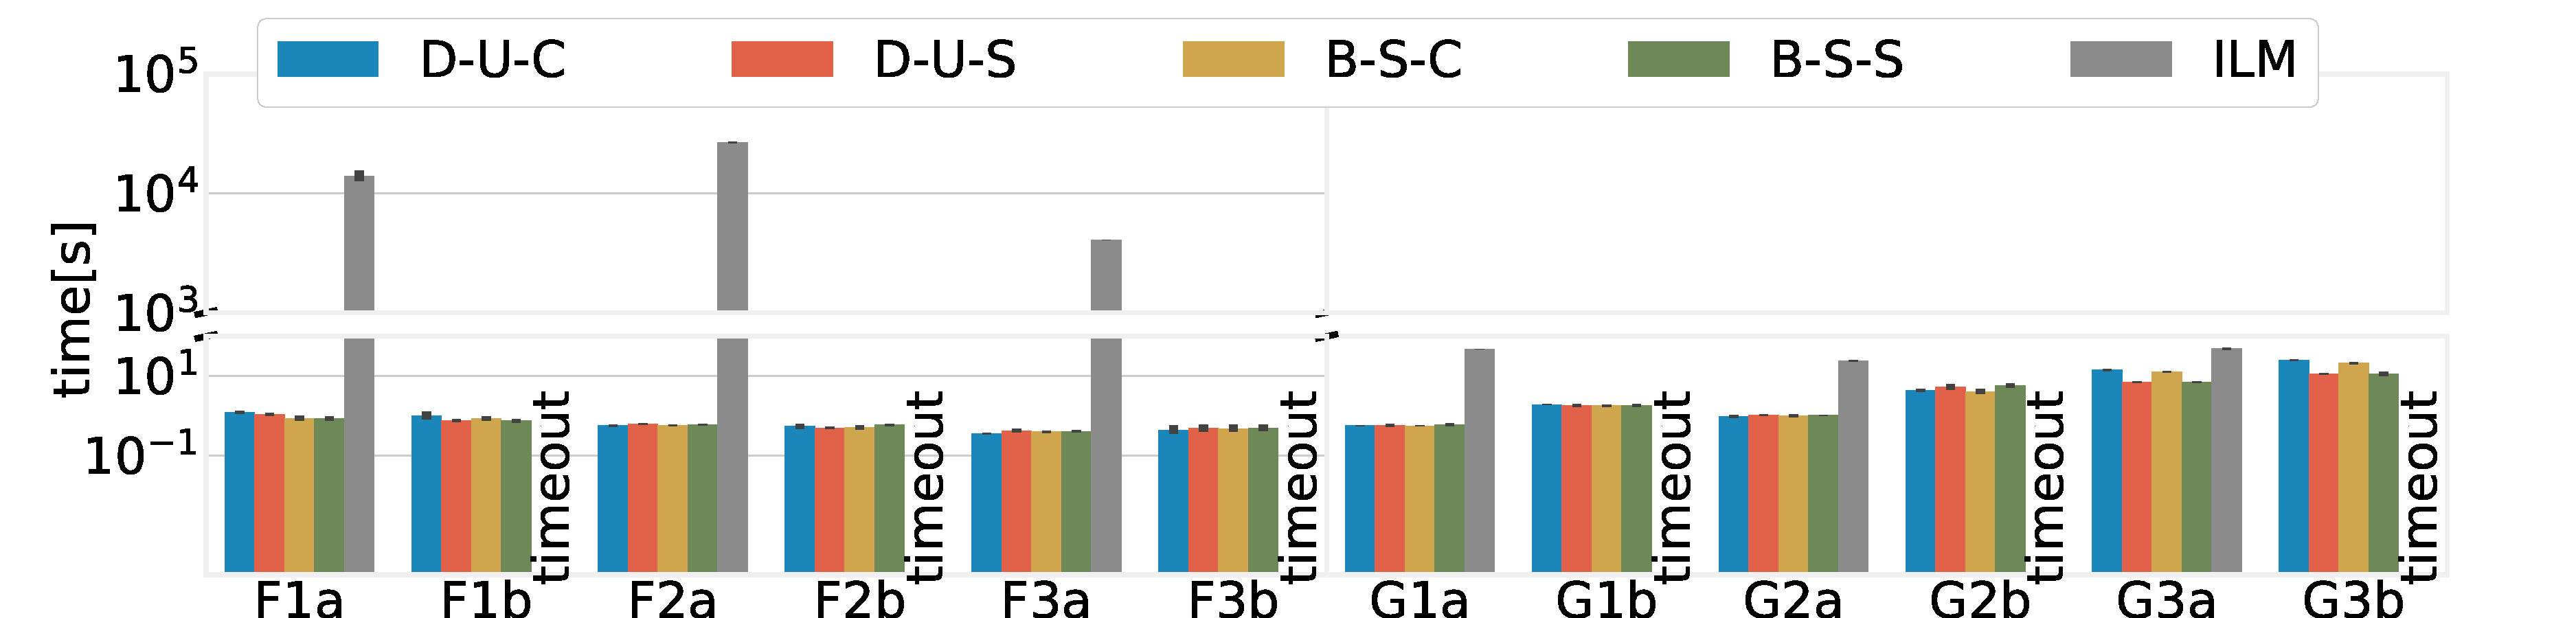
\includegraphics[width=0.95\textwidth]{img/sota_4_broken_new.pdf}
		\vspace{-1em}
		\caption{Runtime comparison with the state of the art.}
	\label{fig:sota}
\end{minipage}
\begin{minipage}[c]{0.29\textwidth}
	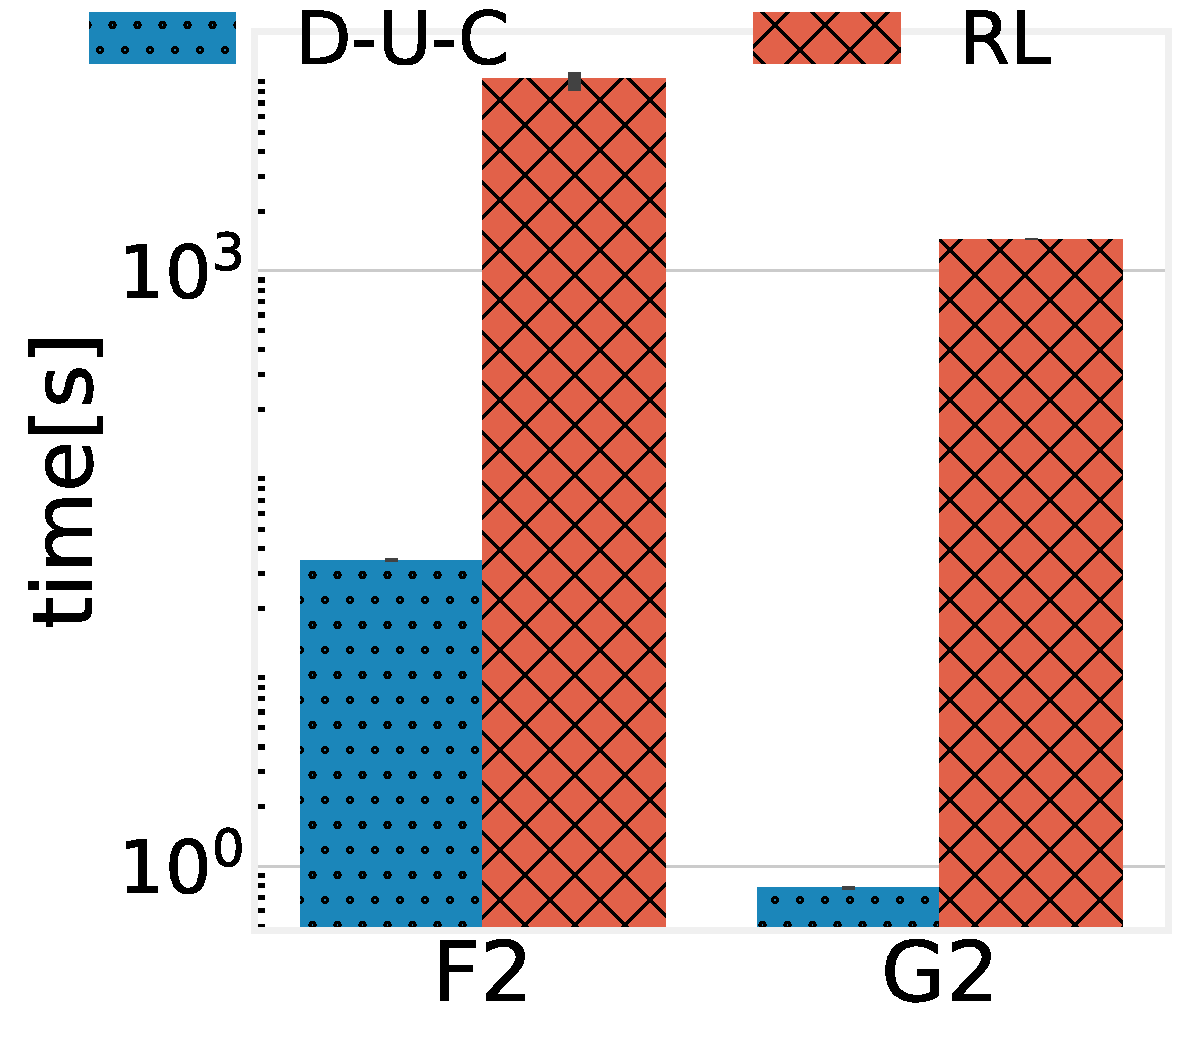
\includegraphics[width=0.65\textwidth]{img/rl_compare.pdf}
	\vspace{-1em}
	\caption{Runtime, RL approach.}
	\label{fig:rl}
\end{minipage}
\vspace{-1em}
\end{figure*}
\sstitle{Measures} We primarily measure the efficiency of event query
discovery in terms of the algorithms' runtime. We report averages over five
experimental runs, including error bars (mostly negligible).
\sstitle{Environment}
We implemented the \sys{} framework in Python. Due to performance issues
of the Java-based version of the IL-Miner and the
absence of a public implementation of the representation learning approach,
we relied on Python-based implementations of the baseline algorithms.
All experiments were conducted on a server with a Xeon 6354 CPU @3,6GHz and
1TB of RAM.
\subsection{State-of-the-Art Comparison}
\label{sec:exp_sota}
First, we compare the runtimes of our algorithms and the
extended IL-Miner, which supports our full query model.
The results in \autoref{fig:sota} show that our algorithms are faster than
the IL-Miner in all cases. For the scenarios based on the finance dataset,
our algorithms are about five orders of magnitude faster. As discussed, we
determined the stream lengths for the $a$ and $b$ scenarios as the
computational limit of the state of the art, i.e., in all $b$ scenarios, the
IL-Miner cannot produce results within 12 hours. The algorithms of the
\sys{} framework enable us to get past this limit in all cases, without a
notable increase in the runtime.
A comparison with the lossy IL-Miner reveals that its improved runtime is traded
for result correctness. The lossy
IL-Miner yields similar runtimes compared to our algorithms, see
\autoref{tab:sota_acc}, yet
it discovers
only a fraction of the queries. That is, with the correct results containing 8
(finance) and 19 (Google) descriptive queries (`Desc'), the lossy IL-Miner
discovers none or only one of them (`Found'), and additionally two and four
queries that are not descriptive (`$\neg$ Desc'). As such, it largely compromises
the result quality not only in terms of descriptiveness, but also in terms of
completeness.
\begin{table}
	\footnotesize
	\caption{Comparison of our algorithms and the lossy IL-Miner.}
	\vspace{-1em}
	\label{tab:sota_acc}
	\begin{tabular}{ c c c c c}
\toprule
Datasets & Avg ${}^{\text{Time Lossy ILM}}/_{\text{Time \sys{}}}$ &
{Desc}(riptive) & Found &
$\neg$
{Desc}\\
\midrule
F1b-F3b & 0.42 & 8 & 0 & 4\\
G1b-G3b & 2.9 & 19 & 1 & 2 \\
\bottomrule
\end{tabular}

	\vspace{-1em}
\end{table}
Finally, we turn to the comparison with the approach based on representation
learning. Since the latter can only discover type queries, we adapted one of our
algorithms (D-U-C) to also return only these queries.
For the datasets F2b and G2b, \autoref{fig:rl} shows the obtained runtime
results, illustrating that our algorithm is at least two orders of magnitude
faster than the baseline algorithm. The effectiveness of query discovery is
summarized in \autoref{tab:rl_compare}. None of the descriptive queries is
discovered by the baseline (`Found'), while only one matching, but not
descriptive query is returned for either scenario (`$\neg$ Desc'). Also, the
construction based on representation learning yields several queries that
are not supported by the stream database (`$\neg$ Matching'). Hence, the
learning-based approach compromises correctness, descriptiveness, and
completeness and, due to high runtimes, is not suitable to address the problem of
event query discovery.
\begin{table}
	\footnotesize
	\caption{Comparison of our algorithms and the RL approach.}
	\vspace{-1em}
	\label{tab:rl_compare}
	\begin{tabular}{ccccc}
\toprule
Dataset & {Desc}(riptive) & Found & $\neg$ {Desc} & $\neg$
Matching\\
\midrule
F2b & 1 & 0 & 1 & 4 \\
G2b & 1 & 0 & 1 & 3 \\
\bottomrule
\end{tabular}

	\vspace{-1em}
\end{table}
\subsection{Sensitivity Analysis}
\label{sec:exp_sensitity}
All of our algorithms show the same worst-case complexity, but incorporate
different design choices. We explore the impact of these choices regarding
properties of stream databases (as introduced in
\autoref{sec:algo_selection}) in a sensitivity analysis.
For the systematically generated stream databases from
\autoref{tab:synt-scenarios}, the results are shown in \autoref{fig:synt_plots}.
Varying the number of streams (E1) leads to generally higher runtimes. As
the size of the database influences the matching of query
candidates, all of our algorithms are effected in the same manner.
An increased length of the streams (E2), as expected (see
\autoref{sec:algo_selection}), has no impact on discovery efficiency. It
does not influence the size of the space of candidate queries to explore.
For the four properties introduced in \autoref{sec:algo_selection} for
algorithm selection, the results
confirm our hypotheses.
\change{A higher number of attributes (E3) favours algorithms that avoid
merging type and pattern queries.
Specifically, D-U-S and D-U-C outperform B-S-S and B-S-C, as merging queries becomes computationally
expensive with more attributes. Increasing the set of
supported attribute values (E4) benefits algorithms that separate the discovery of type and pattern queries.
B-S-S and B-S-C are more efficient under these conditions, due to the
complexity of unified query handling with a large alphabet.
As for the distribution of supported attribute values (E5), D-U-C and B-S-C
perform better due to reduced merge operations.
Conversely, repeated attribute values (E6) favour D-U-S and B-S-S,
as these approaches minimize the search space for pattern queries.}
\change{In sum, our results confirm that the design
choices captured in the \sys{} framework influence the discovery efficiency
as postulated.
The properties of a stream database indeed play a crucial role in
determining which algorithm performs best.}
\begin{figure}
	\centering
	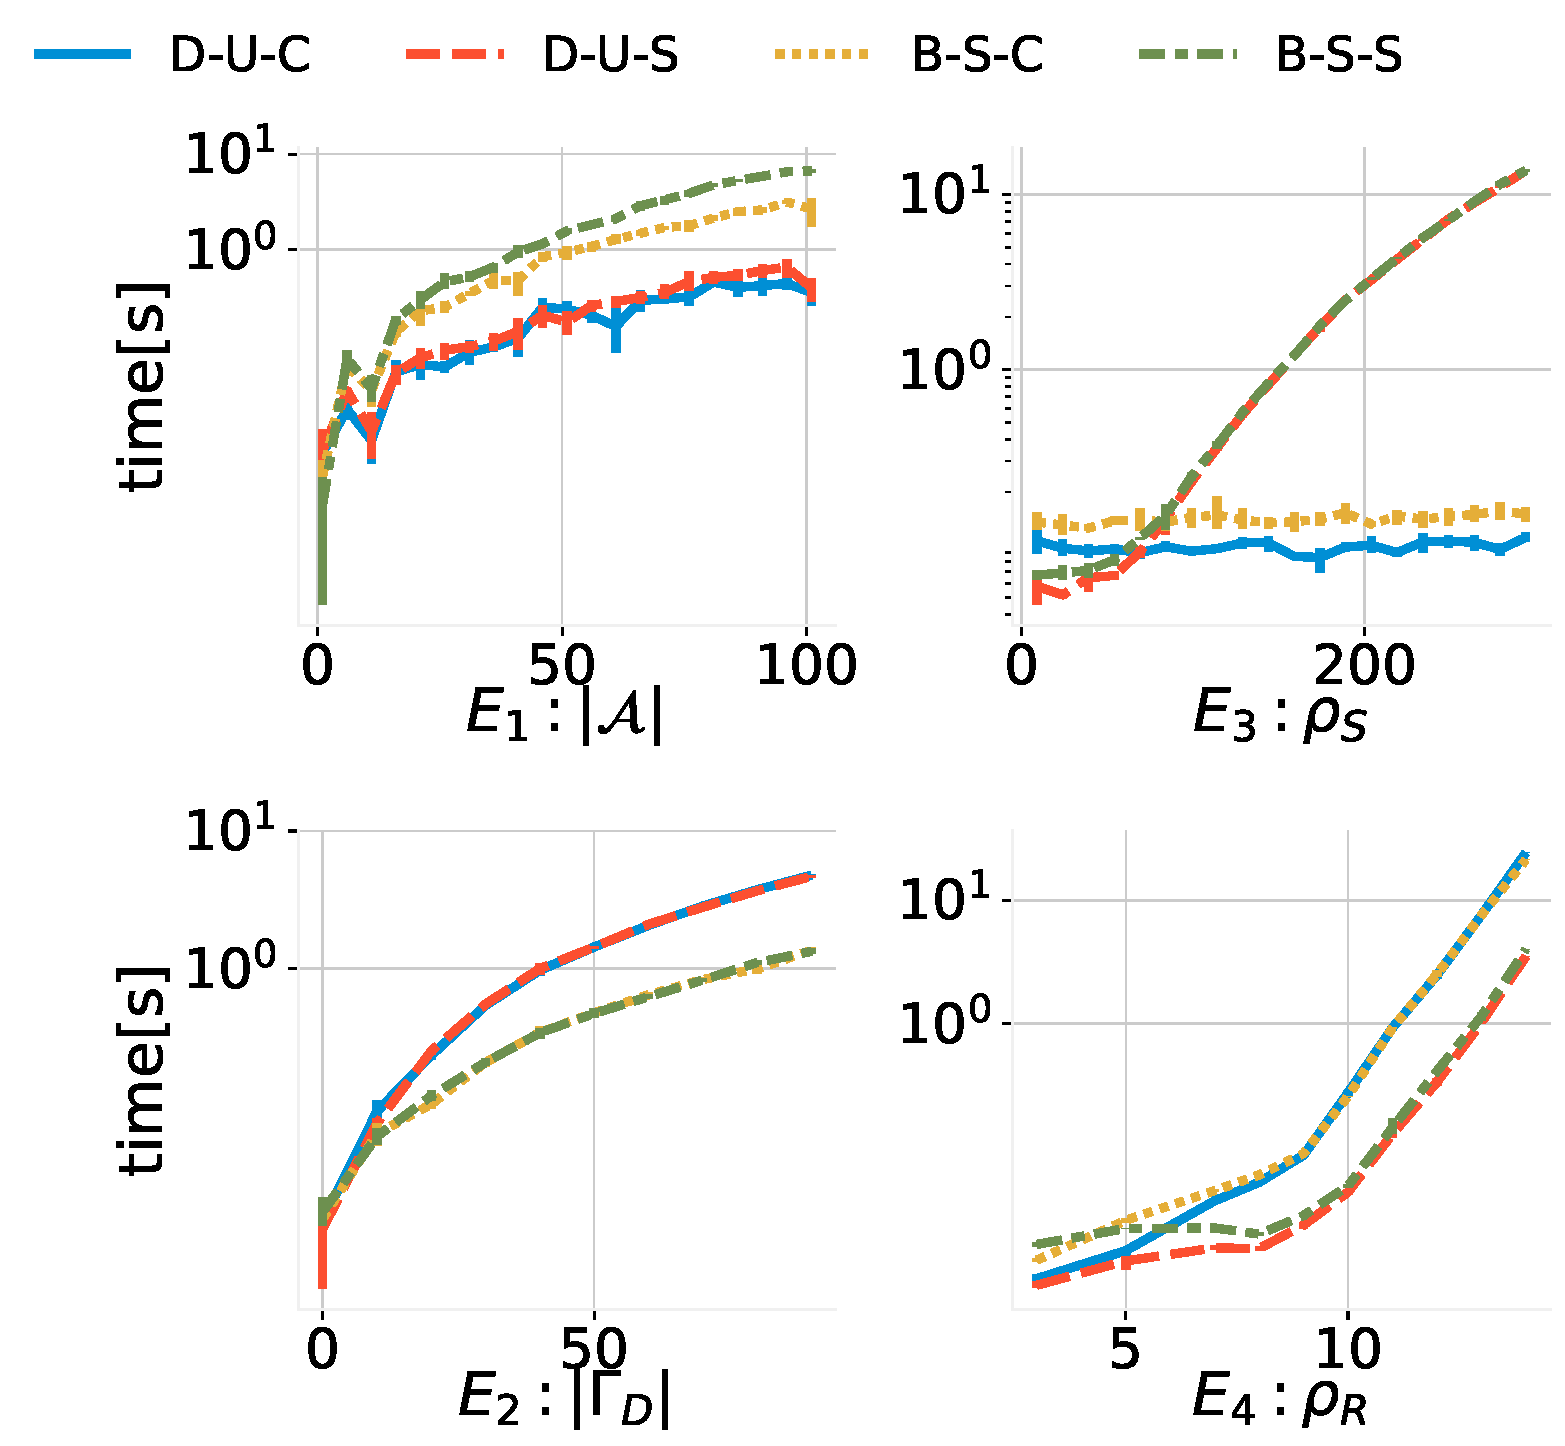
\includegraphics[width=0.95\columnwidth]{img/synt_plots.pdf}
	\vspace{-1em}
	\caption{Sensitivity analysis using synthetic data.}
	\label{fig:synt_plots}
	\vspace{-.5em}
\end{figure}
\subsection{Guidance of Query Discovery}
\label{sec:exp_guidance}
\sstitle{Algorithm selection}
Next, we assess whether the above observations enable us to guide the
selection of a discovery algorithm for the real-world data.
From \autoref{tab:char_corr}, we conclude that the
differences in the number of attributes ($|\mathcal{A}|$) and supported
attribute values ($|\Gamma_D|$) are too small to enable any differentiation,
while the results for the repeated attribute values ($\rho_R$) relate to
an inconclusive value range (see \autoref{fig:synt_plots}). Interestingly,
the measure based on the supported attribute values ($\rho_S$) provides
clues on the runtime performance. For $\rho_S=5$, the algorithms
handling attributes separately (D-U-S and B-S-S) perform much better than
those handling them comprehensively. For $\rho_S>10$, the runtimes of our
algorithms show the opposite trend. Hence, the considered database
properties, assuming that their absolute values provide sufficiently strong
indicators, indeed enable conclusions on the suitability of our algorithms.
\begin{table}[t]
	\footnotesize
	\caption{Correlation of runtime and database properties.}
	\label{tab:char_corr}
	\vspace{-1em}
	\begin{tabular}{cccccccc}
\toprule
\multicolumn{4}{c}{Algorithm Runtime} & \multicolumn{4}{c}{Database
Properties} \\
D-U-C & D-U-S & B-S-C & B-S-S & $\rho_R$ & $\rho_S$ & $|\mathcal{A}|$ & $|\Gamma_D|$ \\
\midrule
18.28 & 26.43 & 17.65 & 26.21 & 6 & 11 & 3 & 2 \\
13.50 & 14.95 & 10.52 & 13.34 & 5 & 17 & 3 & 2 \\
0.65 & 1.39 & 0.88 & 1.68 & 9 & 15 & 3 & 6 \\
259.11 & 364.07 & 226.32 & 366.51 & 10 & 12 & 4 & 1 \\
55.43 & 83.84 & 49.32 & 84.51 & 8 & 10 & 4 & 1 \\
533.90 & 172.54 & 488.45 & 172.37 & 8 & 5 & 4 & 1 \\
\bottomrule
\end{tabular}

	\vspace{-1em}
\end{table}
\sstitle{Feedback mechanisms}
Finally, we tested our mechanisms for feedback on the algorithmic
performance.
First, we assessed whether the exclusion of attribute values may indeed serve
as an abstraction to reduce the discovery runtime.
\autoref{fig:exclude} shows the relative change in
runtimes, when step-wise realizing such an exclusion.
Here, E1 refers to the original database, while for E2-E4, we step-wise
removed the most frequent values of the attribute of the smallest
domain (`volume' for finance, `status' for Google). As expected, the
runtime  decreases. For both datasets, the value
distributions are skewed, so that excluding the most frequent
value (E2) has the largest effect.
Second, we study the abstraction of clustering of attribute values. C1
denotes the original
dataset without clustering. Then, for the Google dataset, we clustered the
`priority' attribute, as adopted in~\cite{reiss2011google} (C2)
and~\cite{reiss2012towards} (C3). For the finance dataset, we clustered the
`close price' into 100 (C2) or 50 (C3)
equally-sized clusters.
\autoref{fig:cluster} highlights that higher numbers of values
within a cluster increase the runtimes. For the finance dataset, the effect
is generally larger and especially affects the algorithms that handle
attributes
comprehensively. However, we
motivated the
abstraction with the desire to increase the result size. For the finance
dataset, we obtain 18 (C1), 30 (C2), and 106 (C3) descriptive queries, while
for the Google dataset, the result includes  202 (C1), 153 (C2), and 298
(C3) queries. We conclude that the expected trend materializes for our data,
even though there is no monotonic relation. The latter is explained
by the fact that clustering may also lead to similar descriptive queries
being merged
into one, which may dominate the effect of having more descriptive queries
due to smaller attribute domains.
\begin{figure}
	\centering
	\begin{minipage}[c]{0.23\textwidth}
		\centering
		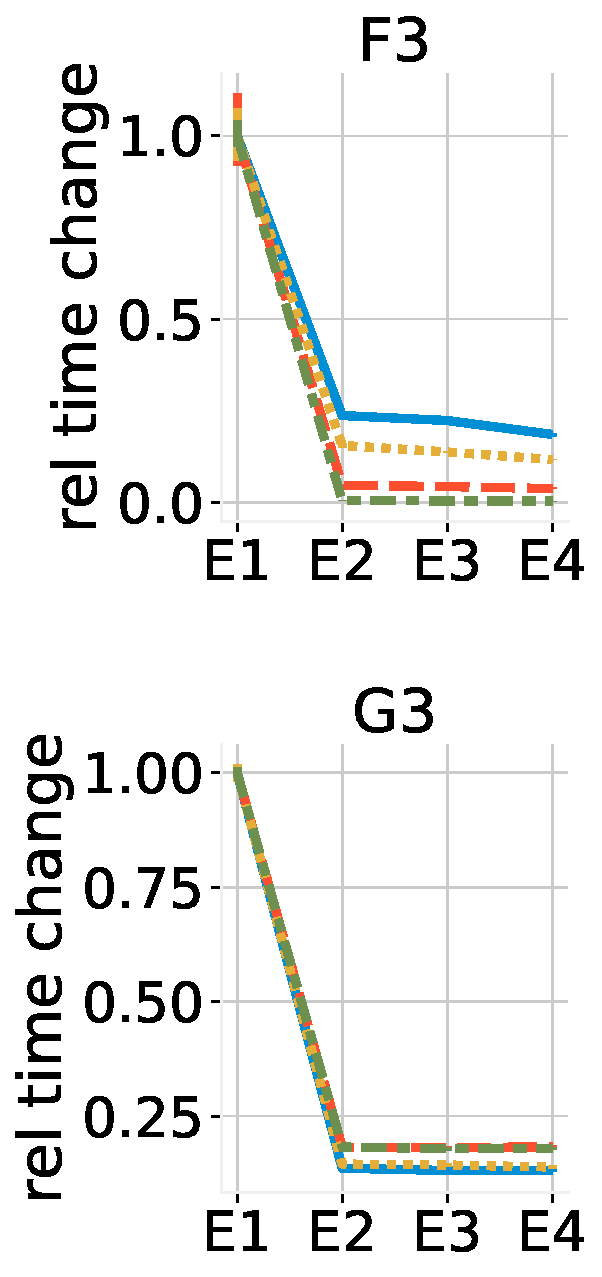
\includegraphics[scale=0.24]{img/exclude.pdf}
		\vspace{-1em}
		\caption{Attr. exclusion.}
		\label{fig:exclude}
	\end{minipage}
	\begin{minipage}[c]{0.23\textwidth}
		\centering
		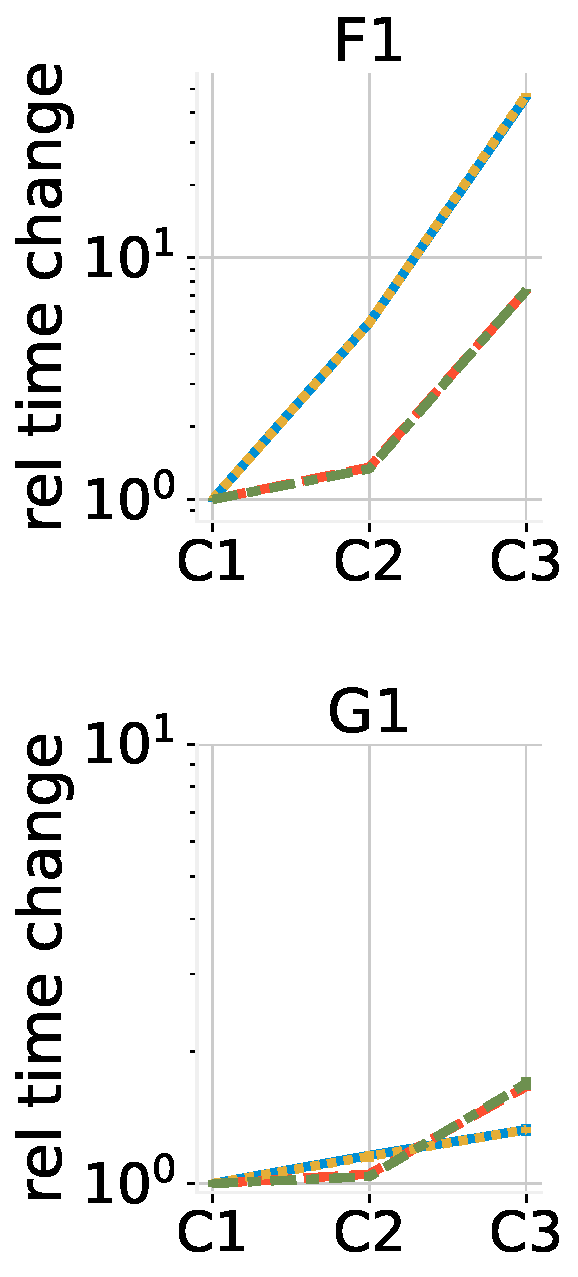
\includegraphics[scale=0.24]{img/cluster.pdf}
		\vspace{-1em}
		\caption{Attr. clustering.}
		\label{fig:cluster}
	\end{minipage}
	\vspace{-1em}
\end{figure}
\section{Related Work}
\label{sec:related_work}
Closest to our work are iCEP~\cite{icep} and the IL-Miner~\cite{ilminer},
which both address the problem of event query discovery based on historic
streams. Yet, both
algorithms take ad-hoc design choices and adopt a restricted query model.
iCEP cannot discover queries, in which attribute values
occur multiple times. This limitation is overcome by the IL-Miner, which,
however, cannot discover queries with query terms containing only
variables. We showed empirically that this lossy version of the IL-Miner
suffers from incomplete results. Also, our algorithms outperform an extended
version of the IL-Miner and extend the set of problem
instances that may be addressed.
Our query model and the notion of descriptiveness is inspired
by~\cite{icdt2022,DBLP:conf/btw/Kleest-Meissner23}. Yet, the discovery
algorithms proposed in~\cite{icdt2022,DBLP:conf/btw/Kleest-Meissner23} are
limited to finding
\emph{some} descriptive queries, not all of them.
Machine learning approaches to anticipate situations of
interest provide an alternative angle to stream-based
monitoring~\cite{yanli2021,ARECEP,autoCEP}. The main drawback of these
methods,
however, is the lack of traceability of the derived
predictions. Using an approach to construct probabilistic state
machines based on representation learning~\cite{yanli2021} in our
evaluation, we observed correctness and completeness issues.
Event query discovery is linked to frequent sequence
mining~\cite{agrawal1995,clospan,bide}, which considers solely
the level of attribute values, though. Our query model embeds a finite
sequence into
another sequence that satisfies certain
constraints. This problem setting is ubiquitous in foundational algorithmic
research, especially in combinatorial string
matching~\cite{DayEtAl2022,KoscheEtAl2022}.
Pattern discovery has also been investigated for
time-series data~\cite{streaming,crossmatch}, which, again, works only  on
attribute values and ignores criteria to correlate events by means of
variables.
\section{Conclusions}
\label{sec:conclusions}
In this paper, we systematically explored the design space
for algorithms that discover event queries from a stream database. We
captured the design choices in the \sys{} framework and instantiated it to
derive four discovery algorithms, which all
provide correct and complete results. Our experiments highlight
that our algorithms outperform the state of the art in event query
discovery, significantly extending the size of the problem instances that
are still tractable. Moreover, we studied the influence of database
properties on the algorithms' efficiency and the discovery result, thereby
providing an angle to improve their applicability.





\begin{acks}
 This work was funded by the German Research
Foundation (DFG), CRC 1404: "FONDA: Foundations of
Workflows for Large-Scale Scientific Data Analysis".

\end{acks}

\clearpage

\bibliographystyle{ACM-Reference-Format}
\bibliography{references}

\clearpage
\appendix
\section{Appendix}
\label{app}

In this appendix, we provide additional details that, due to space
restrictions, could not be included in the main part of the paper. In
particular, this appendix covers the following aspects:
\begin{itemize}[noitemsep,left=1em]
\item A comparison of the query models adopted by different approaches for
event query discovery (\autoref{sec:languages}).
\item Additional experimental results on a comparison of our algorithms with
one that is based on representation learning (\autoref{sec:learning}).
\item A formalization of function \textsc{MergeAttributeQueries} to
merge queries found per attribute (\autoref{sec:alg_merge_attribute}).
\item A formalization of function \textsc{DescriptiveQueries} to select only
the descriptive queries in a set of queries
(\autoref{sec:alg_descriptive_queries}).
\item Formalizations of the D-U-S and B-S-S algorithms as instantiations of
the \sys{} framework (\autoref{sec:alg_further}).
\item A detailed discussion of completeness considerations for our
algorithms (\autoref{sec:completeness}).
\end{itemize}



\subsection{Query Model Comparison}
\label{sec:languages}

We first consider the query model adopted in iCEP~\cite{icep}. It is based
on an notion of events that are typed and carry a set of attribute values.
Queries are defined by operators that filter events, constrain their
attribute values, or require their joint or ordered occurrence, within a
certain time window.

Event query discovery with iCEP is organized in so-called learners, e.g.,
for learning the event types that are considered most relevant as they occur
in all given streams. However, considering the sequence learner to discover
an ordering of events, we note that it is applied solely on the level of
characterizations of events that have been derived in earlier steps. Such
characterizations correspond to query terms in our model. Hence, in
comparison to the algorithms of the \sys{} framework, iCEP is not capable to
discover queries that include the same query term multiple times. For the
database of our running example, see \autoref{ex1}, for instance, the query
$q_1 = \langle (\_,\text{schedule},\_),(\_,\text{schedule},\_)\rangle$
would not be discovered.

The IL-Miner~\cite{ilminer}, in turn, relies on an event and query model
that is close to the one underlying the \sys{} framework. That is, events
have a relational schema and queries define sequences of event variables,
which may be constrained by predicates. Such predicates may require an
attribute value of an event to assume a certain value, or they impose
correlation conditions by requiring the attribute values of two events to be
the same.

The discovery procedure of the IL-Miner first determines so-called relevant
event templates, i.e., sets of predicates that characterize relevant events.
Then, frequent sequence mining is used to extract an order over these
templates. While, this way, the above limitation discussed for iCEP is
avoided, the approach is also more restricted than our algorithms of the
\sys{} framework. In particular, the IL-Miner can only discover queries for
which the events are characterized by particular assignments of attribute
values. Hence, queries that only require the equivalence of attribute values
in events, but do not enforce any specific attribute values, cannot be
discovered. Again, using our example scenario from \autoref{ex1}, for
instance, it would be impossible to discover the query
$q_2 = \langle (\_,x_0,\_),(\_,x_0,\_)\rangle$.



\subsection{Comparison against a Representation Learning Approach}
\label{sec:learning}

To add another perspective, we report on experiments using a representation
learning algorithm for event streams, as introduced in~\cite{yanli2021}. The
approach learns a probabilistic
automaton to capture events and dependencies that indicate a situation of
interest. While the learned automaton is used for stream monitoring
in~\cite{yanli2021}, a query can be extracted from it by enumerating certain
transition paths~\cite{makowsky2012}. While this
approach
yields only type queries, no pattern queries or mixed queries, a comparison
sheds light on the potential of learning-based techniques for event query
discovery.


Since the algorithm can only discover type queries, we adapted one of our
algorithms (D-U-C) to also return only these queries.
This way, the outcome as well as the runtimes become comparable.
For the datasets F2b and G2b, \autoref{fig:rl} shows the obtained runtime
results, illustrating that our algorithm is at least two orders of magnitude
faster than the baseline algorithm. The effectiveness of query discovery is
summarized in \autoref{tab:rl_compare}. None of the descriptive queries is
discovered by the baseline (`Found'), while only one matching, but not
descriptive query is returned for either scenario (`$\neg$ Desc'). Also, the
construction based on representation learning yields several queries that
are not supported by the stream database (`$\neg$ Matching'). Hence, the
learning-based approach compromises correctness, descriptiveness, and
completeness and, due to high runtimes, is not suitable to address the
problem of
event query discovery.



\subsection{Merge Attribute Queries}
\label{sec:alg_merge_attribute}


\begin{figure}[t]
	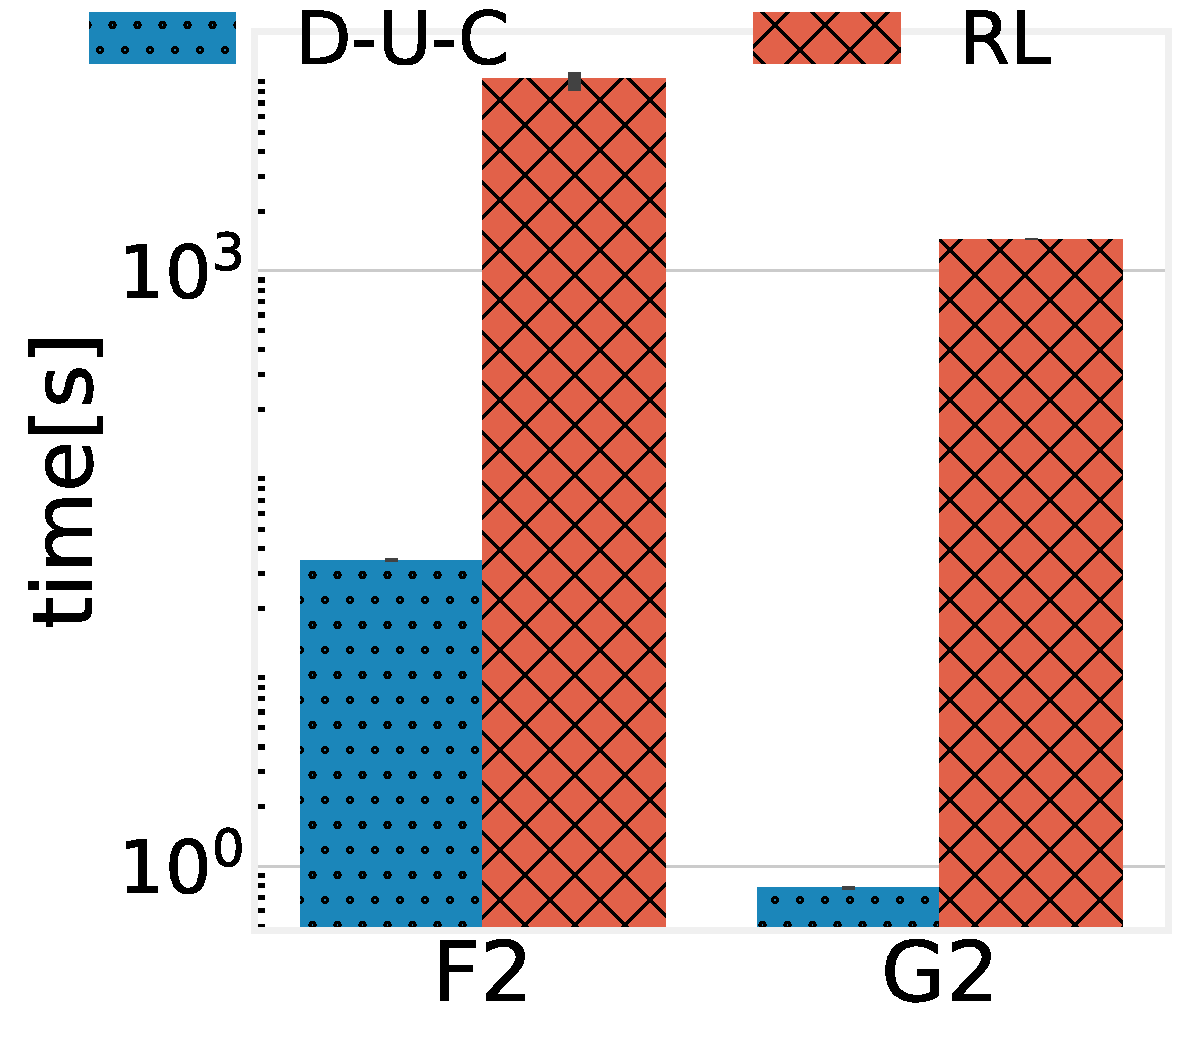
\includegraphics[width=0.45\columnwidth]{img/rl_compare.pdf}
	\vspace{-1em}
	\caption{Runtime, RL approach.}
	\label{fig:rl}
\end{figure}

\begin{table}[t]
	\footnotesize
	\caption{Comparison of our algorithms and the RL approach.}
	\vspace{-1em}
	\label{tab:rl_compare}
	\begin{tabular}{ccccc}
\toprule
Dataset & {Desc}(riptive) & Found & $\neg$ {Desc} & $\neg$
Matching\\
\midrule
F2b & 1 & 0 & 1 & 4 \\
G2b & 1 & 0 & 1 & 3 \\
\bottomrule
\end{tabular}

	%\vspace{-1em}
\end{table}


Our approach to merge queries found per attribute is defined as
\textsc{MergeAttributeQueries} in \autoref{alg-bu-df:mergedomainqueries}.
It takes as input a dictionary of matching queries for each attribute
$Q_{\mathcal{A}}: \mathcal{A} \rightarrow 2^{\mathcal{Q}}$, a parent
dictionary $P$, an event schema $\mathcal{A}$, a stream database $D$, and a
sequence of query variables $\mathcal{X}^<$; and returns a set of merged
queries.

In essence, the algorithm is based on an exhaustive combination of all
combinations of queries sourced from distinct attributes. Each resulting
combination then is handled in several steps:
\begin{itemize}
\item Instance Generation: Initially, for every query found for an
attribute, we systematically
generate all
feasible instances of the query within a single stream of the database.
\item Merge and Translation: Subsequently, we consolidate the instances of
the queries per attribute, and translate them into a unified query.
\item Query Matching: Following the merge, the obtained query is matched
against the stream database. If a match is identified, the merged query is
integrated into the result set.
\end{itemize}

\begin{algorithm}[t]
    \footnotesize
    \caption{\textsc{MergeAttributeQueries}}
    \label{alg-bu-df:mergedomainqueries}
    \KwIn{\, \ Dictionary of matching queries for each attribute
    	$Q_{\mathcal{A}}$,\\
    	\hspace{3em} \,  parent
    	dictionary $P$, event schema $\mathcal{A}$, stream database $D$,\\
    	\hspace{3em} \,  sequence of query variables $\mathcal{X}^<$.}
    %\tcc*{some comment}
    \KwOut{Set of descriptive queries $Q_d$.}
    \BlankLine
    % $n \leftarrow |\mathcal{A}|$\;
    $Q_{m} \leftarrow \emptyset$\;
    $\Gamma_D \gets \{a \in \Gamma \mid \forall \ S \in D: \exists \
	j\in\{1,...,|S|\}, i\in\{1,...,n\}: S[j].A_i = a\}$\;
	\tcc{\scriptsize{All combinations of queries from different
	attributes}}
    $L\leftarrow \bigtimes_{A\in\mathcal{A}}Q_{\mathcal{A}}(A)$\;
     \tcc{\scriptsize{Stream matches dictionary}}
    $T\leftarrow\emptyset$\;

    \ForEach{$(q_1,\ldots,q_n)\in L$}
    {
    		$I \gets \emptyset$\;
    		\lForEach{$q\in \{q_1,\ldots,q_n\}$}{$I(q) \gets \emptyset$}
	        \ForEach{$q \in (q_1,\ldots,q_n)$}
	        {
		\tcc{\scriptsize{Instance positions of query $q$ in $D$}}
		            $I(q) \leftarrow \textsc{GetInstances}(q,D)$\;
		  \If{$\forall q'\in \dom(P): P(q')\neq q $}{
                ${P \leftarrow}$
		\textsc{ChildQueries}($\mathit{q,\mathcal{A},\Gamma_D,P,\mathcal{X}^<,\True}$)\;
          }
          }
	        \tcc{\scriptsize{All
		combinations of instance positions of queries from different
		attributes}}
	        $B \leftarrow \bigtimes_{q_A\in\{q_1,\ldots,q_n\} } I(q_A)$\;
	        \ForEach{$(q'_1,\ldots,q'_n)\in B$}
	        {
	        	\tcc{\scriptsize{Translate instance tuple to query}}
		            $q_{m} \leftarrow
		            \textsc{Instance2Query}((q'_1,\ldots,q'_n),(q_1,\ldots,q_n))$\;
                    ${P \leftarrow}$
		\textsc{ChildQueries}($\mathit{q_m,\mathcal{A},\Gamma_D,P,\mathcal{X}^<,\True}$)\;
		            $q_p \leftarrow P(q_m)$\;
		            $M,T\leftarrow \textsc{Match}(q_m,\mathcal{A},
		            D,q_p,T)$\;
			    \tcc{\scriptsize{Add merged query to result set}}
		            \lIf{$M=\True$}
		            {
                   $Q_{m} \leftarrow Q_{m} \cup \{q_m\}$
			            }
		        }
	    }
    \Return $Q_m$\;
\end{algorithm}


\begin{algorithm}[t]
	\footnotesize
	\caption{\textsc{DescriptiveQueries}}
	\label{descriptivequeries}
	\KwIn{\, \ Set of queries $Q$, supported alphabet
		$\Gamma_D$, event schema $\mathcal{A}$,\\
		\hspace{3em} \,  sequence of query variables $\mathcal{X}^<$ over
		the set of query variables $\mathcal{X}$.}
	%\tcc*{some comment}
	\KwOut{Set of descriptive queries $Q_d$.}
	\BlankLine
	$Q_n\leftarrow \emptyset$\;
	\tcc{\scriptsize For each query $q$ in the query set $Q$, create queries
		which are less strict and therefore not descriptive}
	\ForEach{$q \in Q$}{
		$R \gets \emptyset$\;
		\lForEach{$s\in \Gamma_D\cup\mathcal{X}$}
		{$R(s)\gets \emptyset$}
		\ForEach{$i\in\{1,\dots,|q|\}$}{
			\label{alg10_1_start}
			\ForEach{$A\in\mathcal{A}$}{
				\If{$q[i].A \in \Gamma_D\cup\mathcal{X}$}
				{$q_n \gets q$\;
					$q_n[i].A \gets \_$\;
					$Q_n \gets Q_n\cup \textsc{Normalform}(q_n)$\;
					$R(q[i].A)\gets R(q[i].A)\cup \{i\} $\;
				}

			}
			\label{alg10_1_end}
		}
		\ForEach{$s\in\dom(R)$}{
			\If{$s\in\mathcal{X} \land |R(s)|\geq4$}{
				\label{alg10_2_start}
				\tcc{\scriptsize Find all combinations of partial
				replacements
					of variable $s$ in query $q$}
				$G\gets \textsc{GenerateReplacements}(q,s)$\;
				$Q_n \gets Q_n\cup G$\;
			}
			\label{alg10_2_end}
			\If{$s\in\Gamma_D \land |R(s)|\geq2$}
			{
				\label{alg10_3_start}
				\tcc{\scriptsize Find all combinations of partial and
				complete
					replacement of attribute type $s$ in query $q$}
				$G\gets \textsc{GenerateReplacements}(q,s)$\;
				% $q_n\gets q.\textsc{Replace}(s,x) |
				%x\in\mathcal{X}^<,R(x)=0$\;
				$Q_n \gets Q_n\cup G$\;
			}
			\label{alg10_3_end}
		}
	}
	$Q_d\leftarrow Q\backslash Q_n$\label{alg10_sub}\;
	\Return $Q_d$\;
\end{algorithm}

\subsection{Descriptive Queries}
\label{sec:alg_descriptive_queries}

Our approach to select only the descriptive queries in a set of queries is
given as \textsc{DescriptiveQueries} in \autoref{descriptivequeries}. Given
a set of queries $Q$, a supported alphabet
$\Gamma_D$, an event schema $\mathcal{A}$, and a sequence of query variables
$\mathcal{X}^<$ with $\mathcal{X}$ as the underlying set of query variables,
it proceeds as follows. We iterate over each
query $q$ within the given set and, for each query, generate queries that
are less specific than~$q$.
We generate less specific queries in three different ways:
\begin{itemize}
\item Replace each symbol (variable or attribute value) within the query by
the placeholder (\autoref{alg10_1_start}-\ref{alg10_1_end}). For every
replacement, a new non-descriptive query is added
to the set of non-descriptive queries $Q_n$.
\item Partially replace variables that appear at least four times within a
query by a new variable that is not used in query $q$
(\autoref{alg10_2_start}-\ref{alg10_2_end}).
\item Partially and completely replace attribute types that appear at least
twice within the given query  (\autoref{alg10_3_start}-\ref{alg10_3_end}).
\end{itemize}
At the end, we calculate the set of descriptive queries $Q_d$ by subtracting
all queries in $Q_n$ from the given set of queries $Q$ (\autoref{alg10_sub}).

The above approach relies on function \textsc{Normalform}, which checks, if
a variable occurs
at least twice, and otherwise replaces it with the placeholder $\_$. Second,
it restores the order of the variables, such that the first occurrences of
the variables appear in the same order in the query $q$ as they do in
$\mathcal{X}^<$.

%\examplebox{Example - Merging Attribute Queries}{
\begin{example}
	\label{ex:merge}
	Let us consider stream $S_2$ from \autoref{ex1}, the following queries
	per
	attribute, and their matching instances within the stream:



	\begin{center}
		\smallskip
		{\footnotesize
			\begin{tabular}{lll}
				\toprule
				Attribute & Query &  Positions \\
				\midrule
				Job Id & $\varepsilon, q_1=\langle (2,\_,\_) \rangle$   &
				$(e_{21})$, $(e_{23})$  \\
				Status   & $\varepsilon, q_2=\langle (\_,\text{schedule},\_)
				(\_,\text{schedule},\_) \rangle$ & $(e_{21}, e_{22})$   \\
				Priority   & $\varepsilon, q_3=\langle (\_,\_,\text{low})
				\rangle$ & $(e_{21})$, $(e_{23})$   \\
				\bottomrule
		\end{tabular}}
	\end{center}
	The combination of queries found for different attributes leads to the
	following set:
	$$\{(q_1,q_2,q_3), (q_1,q_2,\varepsilon), (q_1,\varepsilon,q_3),
	(\varepsilon,q_2,q_3),$$ $$(q_1,\varepsilon,\varepsilon),
	(\varepsilon,\varepsilon,q_3),
	(\varepsilon,q_2,\varepsilon),(\varepsilon,\varepsilon,\varepsilon)\}. $$
	The connection of the different position for the query tuple
	$(q_1,q_2,q_3)$ leads to the following merged queries:
	\begin{align*}
		&\langle (2,\text{schedule},\text{low}),(\_,\text{schedule},\_)
		\rangle \\
		&\langle
		(\_,\text{schedule},\_),(\_,\text{schedule},\_),(2,\_,\text{low})
		\rangle \\
		&\langle
		(2,\text{schedule},\_),(\_,\text{schedule},\_),(\_,\_,\text{low})
		\rangle \\
		&\langle
		(\_,\text{schedule},\text{low}),(\_,\text{schedule},\_),(2,\_,\_)
		\rangle
	\end{align*}
	which then have to be matched against the complete stream database.
	This process would have to be repeated for all combinations of query
	tuples to get all possible merged queries.
%}
\end{example}

Moreover, function \textsc{GenerateReplacements} takes as input a query $q$
and a symbol $s$, i.e., an attribute value or a variable that is to be
replaced by a variable, which is not used in the query.
The replacement routine first iterates through the number of symbols that can be replaced. In case of a variable (an attribute value) it is $[2,R(s)-2]$ ($[2,R(s)-1]$).
Then, for each group size, it finds all combinations of possible replacements for the current query $q$.

For example, let $s$ be a variable and $R(s)$=5. Let the positions of $s$
within the query be $[1,2,3,4,5]$.
Then the possible group sizes are 2 and 3.
For group size 2, there are $\binom{5}{2}=10$ combinations: $
(1,2),(1,3),\dots, (4,5)$.
For group size 3, there are $\binom{5}{3}=10$ combinations: $
(1,2,3),(1,2,4),\dots, (3,4,5)$.
For each of the calculated positions, $s$ is replaced by the same variable $x$ which is not
used in $q$.
The time complexity of the \textsc{GenerateReplacements} function is exponential,
$O(2^{R(s)})$, due to the generation of all combinations of replacements.
However, in practice, this complexity can be managed by typical constraints on
the values of $R(s)$ in the dataset and by applying optimizations to limit
the number of combinations generated.

The result is a set of
queries which are less specific than query $q$ and, therefore, not
descriptive.



\subsection{D-U-S \& B-S-S}
\label{sec:alg_further}

\sstitle{D-U-S: DFS, pattern-type unified, attribute separated}
As mentioned, the D-U-S algorithm, presented in \autoref{alg-bu-df-ds}, is a
variant of the D-U-C algorithm, which also
employs DFS and constructs queries in a unified manner.
It discovers queries separately per attribute, before merging
them to obtain the
final result. The sets of queries per attribute are maintained in a
dictionary $Q_{\mathcal{A}}: \mathcal{A} \rightarrow 2^{\mathcal{Q}}$, i.e.,
$Q_{\mathcal{A}}(A)$ is the set of queries found for attribute $A\in
\mathcal{A}$. The algorithm first constructs the projections of the streams
on the attribute (\autoref{alg9:projection}), which are then used to run the
D-U-C algorithm (\autoref{alg9:mining}). Note that setting flag $b$ to
$\False$ means that the D-U-C algorithm will return all found queries, not
only those that are descriptive. The queries discovered per attribute are
then merged, as detailed above, before the non-descriptive queries are
removed from the result.


\sstitle{B-S-S: BFS, pattern-type separated, attribute separated}
The B-S-S algorithm is defined in \autoref{alg-bu-bf-ds}. It is a variant of
B-S-C, adopting BFS and the separated
discovery of type queries and pattern queries. Yet, it first considers
queries per attribute, which are again collected in a
dictionary $Q_{\mathcal{A}}: \mathcal{A} \rightarrow 2^{\mathcal{Q}}$,
before merging them using the algorithm introduce above. As such, it
adopts the strategy explained above for D-U-S, just with B-S-C as the base
algorithm.



\begin{algorithm}[t]
	\footnotesize
	\caption{D-U-S}
	\label{alg-bu-df-ds}
	\KwIn{\, \ Stream database $D$, event schema $\mathcal{A}$, sequence of
		query var. $\mathcal{X}^<$.}
	\KwOut{Set of descriptive queries $Q$.}
	\BlankLine
	\tcc{\scriptsize Set of queries and parent dict. per
		attribute}
	$\mathit{Q_{\mathcal{A}}, P_{\mathcal{A}} \leftarrow \emptyset}$\;
	\ForEach{$A\in\mathcal{A}$}{$Q_{\mathcal{A}}(A), P_{\mathcal{A}}(A)
		\leftarrow \emptyset,\emptyset$\;}
	\tcc{\scriptsize Use D-U-C to discover queries per attribute}
	\ForEach{$A\in\mathcal{A}$}{
		\label{alg9:projection}
		$D_A \leftarrow \{\langle (e_1.A), \dots, (e_{l}.A)\rangle
		\mid \langle e_1,\ldots, e_l\rangle \in D \}$\;
		\label{alg9:mining}
		$Q_{\mathcal{A}}(A),P_{\mathcal{A}}(A)\leftarrow
		\textsc{D-U-C}(D_A,(A),\mathcal{X}^< ,\False)$\;
	}

	$P \leftarrow \cup_{A\in\mathcal{A}} P_\mathcal{A}(A)$\;
	\tcc{\scriptsize Merge queries found per attribute}
	$Q \leftarrow
	\textsc{MergeAttributeQueries}(Q_{\mathcal{A}},P,\mathcal{A},D,\mathcal{X}^<)$\;
	%%{\scriptsize \tcp*{\autoref{alg-bu-df:mergedomainqueries}}}
	$Q \leftarrow
	\textsc{DescriptiveQueries}(Q,\Gamma_D,\mathcal{A},\mathcal{X}^<)$\;
	%%{\scriptsize \tcp*{\autoref{alg-bu-df:mixedqueries}}}
	\Return $\mathit{Q}$\;
	%\textbf{break};
\end{algorithm}
\begin{algorithm}[t]
	\footnotesize
	\caption{B-S-S}
	\label{alg-bu-bf-ds}
	\KwIn{\, \ Stream database $D$, event schema $\mathcal{A}$, sequence of
	query var. $\mathcal{X}^<$.}
	\KwOut{Set of descriptive queries $Q$.}
	\BlankLine
	\tcc{\scriptsize Set of queries and parent dict. per
		attribute}
	$\mathit{Q_{\mathcal{A}}, P_{\mathcal{A}} \leftarrow \emptyset}$\;
	\ForEach{$A\in\mathcal{A}$}{$Q_{\mathcal{A}}(A), P_{\mathcal{A}}(A)
		\leftarrow \emptyset,\emptyset$\;}
	\tcc{\scriptsize Use B-S-C to discover queries per attribute}
	\ForEach{$A\in\mathcal{A}$}{
		\label{alg10:projection}
		$D_A \leftarrow \{\langle (e_1.A), \dots, (e_{l}.A)\rangle
		\mid \langle e_1,\ldots, e_l\rangle \in D \}$\;
		\label{alg10:mining}
	        $Q_{\mathcal{A}}(A),P_A\leftarrow
	\textsc{B-S-C}(D_A,(A),\mathcal{X}^< ,\False)$\;
	}

	$P \leftarrow \cup_{A\in\mathcal{A}} P_\mathcal{A}(A)$\;
	\tcc{\scriptsize Merge queries found per attribute}
	$Q \leftarrow
	\textsc{MergeAttributeQueries}(Q_{\mathcal{A}},P,\mathcal{A},D,\mathcal{X}^<)$\;
	%%{\scriptsize \tcp*{\autoref{alg-bu-df:mergedomainqueries}}}
	$Q \leftarrow
	\textsc{DescriptiveQueries}(Q,\Gamma_D,\mathcal{A},\mathcal{X}^<)$\;
	%%{\scriptsize \tcp*{\autoref{alg-bu-df:mixedqueries}}}
	\Return $\mathit{Q}$\;
\end{algorithm}


\subsection{Completeness}

\label{sec:completeness}
While we highlighted several arguments regarding completeness of our
algorithms already in \autoref{sec:realizations}, we now turn to a more
detailed discussion.
The functions that are relevant for an assessment of completeness, i.e.,
that determine that all potentially matching queries are generated at least
once to be checked for matching, are mainly: The algorithms for generating
query candidate, for merging pattern and type queries, and for merging
attribute queries.
We will discuss their completeness in dedicated subsections, i.e.,
\ref{sec:comp-candidates}, \ref{sec:comp-tp}, and \ref{sec:comp-att}.


\subsubsection{Query Candidate Generation}
\label{sec:comp-candidates}
Given a matching query (which, initially, is the empty query in all of our
discovery algorithms), new queries are generated following
a dedicated set of rules, which ensure that each potentially matching query
is generated exactly once:
\begin{enumerate}
	\item \textbf{New variables} are added to a query
	in two locations.  The first one concerns a placement after the first
	position of the last
	inserted variable. The second one concerns the position after the last
	inserted type.
	\item An \textbf{existing variable} is added to a query, only if this
	variable was
	the last inserted symbol. If this is the case, then it can be placed
	at any position after the last occurrence of this variable.
	\item A \textbf{new type} is added to the query  after the first
	position of the last inserted variable, or after the last position
	of any type.
\end{enumerate}
Recalling that the candidate generation always starts with the empty query,
it follows directly that all candidates can be generated based on the above
rules.

As such, the questions becomes if the above rules are correctly realized in
\autoref{alg-bu-df:childquery}. The three rules mentioned
above are implemented as follows: When inserting a new variable, first the
variable is instantiated.
Then, the algorithm iterates over each attribute. For each attribute,
we call the \textsc{Next}-Function which returns all helper queries
with possible first positions for the newly added variable. For all the
generated helper queries the \textsc{Next}-Function is called again
to determine the new candidate queries which are added to the
set of candidate queries.

To insert an existing variable again, we first check whether it
was the last inserted symbol.
Then, we determine the attribute of the variable and generate
new query candidates by calling the \textsc{Next}-Function.

Finally, to generate queries adding a new type, we again iterate
over all the attributes. For each attribute, we consider the
supported attribute values. For each supported attribute value,
the \textsc{Next}-Function is called, and the resulting queries
are added to the set of candidates.

The \textsc{Next}-Function iterates over the query terms starting
with the query term at position $s$ until the last query term of the query.
Then, per query term generates up to two new candidate queries:
First it checks whether the current attribute in the query term
is a placeholder. If this is the case, then it creates a new query
in which the current symbol is added to the attribute of the
current query term. Second it creates a new query by creating
a new query term right after the current one which only contains
the current symbol at the corresponding attribute and all the
other attributes are set as placeholders.



\subsubsection{Merge Pattern and Type Queries}
\label{sec:comp-tp}
To initalize the merging progress for all pairs of
type and pattern queries, for each of their parent queries $q$.
a 4-tuple is added to the queue of queries to be merged.
The 4-tuple consists of a type query $q_t$, a pattern or mixed query
$q_p$, a mixed query $q_m$ and an evolved query $q_e$. For the
initialization the tuple is set to
$(q_t, q_p, \langle\varepsilon\rangle, q)$
For each such tuple the function \textsc{MergeMixedQueries} is
called which is where the actual merging process takes place.

First the function calculates the starting position from which on
the mixed query can be extended.
If the evolved query is a type query then new merged queries are
generated by inserting the query term after the last occurence of another
type or attribute value,
adding each such generated query to the set of mixed queries.
It also checks whether the type to be added can be merged to an existing
query term in $q_m$.
If the evolved query is not a type query the function first checks
whether all query terms for either the type query or the pattern
query have already been incorporated into the mixed query.
If this is the case then starting from that position, the remaining
query terms of the eluded query are added to the end of the mixed query.
In a second step the function tries insert the current last position of
$q_p$ into the current query term of $q_m$. If this can be done
a new mixed query is generated which merges the query term and adds
the remaining query terms of the evolved query $q_e$.

For the 4-tuples created in the intialization
(\autoref{alg3:init_start}), The set of candidate queries
will either contain a type query
with one query term and one placed attribute value
(if $q_e$ is a type query) or $q_e$ if it is a pattern query.
The returned query candidates are matched and new
4-tuples are added to the queue accordingly.
For the initializiation tuples, the matching is obviously $\True$.
The next 4-tuples added to the queue are
$(q_e, q_p, q_n, q)$, where $q$ is either the empty query or one
of the parents of $q_p$ ($q_t$) if $q_e$ is a type query (pattern query).

Since $q_e$ is always a parent query we pass through all queries until
reaching the empty query.
This way it is assured that all possible queries are generated.


\subsubsection{Merge Attribute Queries}
\label{sec:comp-att}
The function first generates all combinations on $n$-tuples
for the matching attribute queries, such that in each $n$-tuple there
is a query from each attribute and $n$ being the number of
attributes. A valid query for each attribute is also the empty query.

For each $n$-tuple new possible mixed query candidates are generated
using the following procedure:
A function $I$ is called for each attribute query which returns
all the mappings of the query for each stream. For each stream
a list of $k$-tuples is returned, where $k$ is the number
of query terms for the current attribute query and each $k$-tuple
is a match of the query on that stream.

Then for one stream, we calculate all combinations of the different
$k$-tuples of the $n$ attribute queries. Each combination contains
one $k$-tuple from each attribute query in the current $n$-tuple.

It is sufficient to consider the instances of one stream, since
all matching queries necessarily need to match every stream.
This also means that only those queries present in one stream
are possible candidates to match the whole stream.

The resulting combinations of instance tuples are then
translated (if possible) to mixed queries and if they match
are added to the set of mixed queries.


\end{document}
\endinput
